% VLDB template version of 2020-03-05 enhances the ACM template, version 1.7.0:
% https://www.acm.org/publications/proceedings-template
% The ACM Latex guide provides further information about the ACM template
\documentclass[sigconf, nonacm]{acmart}
%% The following content must be adapted for the final version
% paper-specific

\usepackage{color}
\usepackage{enumitem}
\usepackage{float}
\usepackage{balance}% for  \balance command ON LAST PAGE  (only there!)
\usepackage{algorithm, algorithmicx}
\usepackage[noend]{algpseudocode}
\usepackage{tabu}
\usepackage{balance}
\usepackage{booktabs}
\usepackage{graphicx}
\usepackage{subfigure}
%\usepackage{times}
\usepackage{stfloats}
\usepackage{url}
\usepackage{comment}
\usepackage{amsmath}
\usepackage{makecell}
\usepackage{xcolor}


\newcommand\vldbdoi{XX.XX/XXX.XX}
\newcommand\vldbpages{XXX-XXX}
% issue-specific
\newcommand\vldbvolume{14}
\newcommand\vldbissue{1}
\newcommand\vldbyear{2020}
% should be fine as it is
\newcommand\vldbauthors{\authors}
\newcommand\vldbtitle{\shorttitle}

%
\newtheorem{problem}{Problem}
\newtheorem{lemma}{Lemma}
\newtheorem{theorem}{Theorem}
\newcommand{\Bo}[1]{{\color{red} Bo: #1}}
% \newcommand{\QM}[1]{{\color{blue} QM: #1}}
\newcommand{\QM}[1]{{\color{blue}{#1}}}

\newcommand{\D}{\mathsf{T}}
\newcommand{\V}{\mathsf{V}}
\newcommand{\oR}{\mathsf{R}}
\newcommand{\MU}{\mathsf{U}}
\newcommand{\vats}{\mathsf{VFGS}}
\newcommand{\rand}{\mathsf{RAND}}
\newcommand{\full}{\mathsf{FULL}}
\newcommand{\avats}{\mathsf{VFGS}^{+}}
\newcommand{\cavats}{\mathsf{VFGS}^{+}\mathsf{CE}}
\newcommand{\sz}{\textsf{Shenzhen}}
\newcommand{\pt}{\textsf{Porto}}
\newcommand{\trim}{\vspace{-2mm}}

\newcommand{\stitle}[1]{\vspace*{0.4em}\noindent{\bf #1:\/}}
\newcommand{\sstitle}[1]{\vspace*{0.4em}\noindent{\bf #1\/.}}


\newcommand{\squishlist}{
 \begin{list}{$\bullet$}
 { \setlength{\itemsep}{0pt}
   \setlength{\parsep}{3pt}
   \setlength{\topsep}{3pt}
   \setlength{\partopsep}{0pt}
   \setlength{\leftmargin}{1.2em}
   \setlength{\labelwidth}{1em}
   \setlength{\labelsep}{0.6em}
 }
}
\newcommand{\squishend}{
 \end{list}
}

\settopmatter{printfolios=true}





\begin{document}
\title{Visual Fidelity Guaranteed Sampling for \\ Large Trajectory Data Visualization}

%\author{Qiaomu Shen$^{*}$,\quad Chuan Yang$^{*}$,\quad Chaozu Zhang$^{*}$,\quad Dan Zeng$^{\dag}$, \quad Wei Zeng$^{\ddag}$, \quad Bo Tang$^{*}$}

\affiliation{
  \institution{Qiaomu Shen$^{\dag}$,\quad Chuan Yang$^{\dag}$,\quad Chaozu Zhang$^{\dag}$,\quad Dan Zeng$^{\ddag}$, \quad Wei Zeng$^{\$}$, \quad Bo Tang$^{\dag}$}
  \institution{$^{\dag}$ Department of Computer Science and Engineering, Southern University of Science and Technology}
  \mbox{qshen@connect.ust.hk, \{11612732@mail,11712021@mail,tangb3@\}sustech.edu.cn} \\
  \institution{$^{\ddag}$ Electrical Engineering, Mathematics and Computer Science, University of Twente}
  \institution{$^{\$}$ Shenzhen Institutes of Advanced Technology, Chinese Academy of Sciences}
  \mbox{d.zeng@utwente.nl, zengwei81@gmail.com}
  %\email{{{11711004, 11712532, 11613015}@mail.,tangb3@}sustech.edu.cn}
  %\mbox{qshen@connect.ust.hk, \{11612732@mail,11712021@mail,tangb3@\}sustech.edu.cn, d.zeng@utwente.nl, zengwei81@gmail.com}
}

\renewcommand{\shortauthors}{Qiaomu Shen, et al.}
\renewcommand{\shorttitle}{Paper ID: xxx}

%% The abstract is a short summary of the work to be presented in the
%% article.
\begin{abstract}
Visualizing large-scale trajectory data is the core subroutine in many smart city applications, e.g., traffic management, route recommendation.
However, it suffers from limited rendering capability and visual clutter issues.
Sampling can effectively mitigate the issues, yet existing methods have an attenuating effect on visual fidelity.
In this work, we propose visual fidelity guaranteed sampling techniques for line-based visualization of large trajectories.
We first define a pixel-based fidelity loss function to capture the visual difference between two visualizations.
We prove that it is NP-hard to select a sized-$k$ subset of trajectories with minimal visual fidelity loss.
Next, we devise an approximation algorithm $\vats$ with a suite of optimization techniques, which returns fidelity-guaranteed visualizations efficiently.
Moreover, we propose $\avats$ which improves the effectiveness of $\vats$ by taking data distribution and human perception into consideration.
We conduct extensive experimental studies to demonstrate the effectiveness and efficiency of our methods on real-world trajectory datasets.
In addition, comprehensive user studies further illustrate the superiority of our proposals in various applications, e.g., traffic flow comparison, and reachable route inspection.
\end{abstract}

\maketitle


\trim


\begingroup\small\noindent\raggedright\textbf{PVLDB Reference Format:}\\
\shortauthors. Visual Fidelity Guaranteed Sampling for Large Trajectory Data Visualization. PVLDB, \vldbvolume(\vldbissue): \vldbpages, \vldbyear.\\
\href{https://doi.org/\vldbdoi}{doi:\vldbdoi}
\endgroup

\trim \trim \trim

\begingroup
\renewcommand\thefootnote{}\footnote{\noindent
This work is licensed under the Creative Commons BY-NC-ND 4.0 International License. Visit \url{https://creativecommons.org/licenses/by-nc-nd/4.0/} to view a copy of this license. For any use beyond those covered by this license, obtain permission by emailing \href{mailto:info@vldb.org}{info@vldb.org}. Copyright is held by the owner/author(s). Publication rights licensed to the VLDB Endowment. \\
\raggedright Proceedings of the VLDB Endowment, Vol. \vldbvolume, No. \vldbissue\ %
ISSN 2150-8097. \\
\href{https://doi.org/\vldbdoi}{doi:\vldbdoi} \\
}\addtocounter{footnote}{-1}\endgroup
%%% VLDB block end %%%

\section{Introduction}\label{sec:intro}
Nowadays, the {ubiquitous} location-acquisition devices lead to an explosive increase of movement data (a.k.a. GPS trajectories) {for} urban moving objects, e.g., {vehicles}, sharing bikes, and pedestrians.
Trajectory {visualization has} been employed in many smart city applications, e.g.,  traffic management~\cite{wang2014visual}, urban planning~\cite{tang2017efficient}, route recommendation~\cite{zheng2011learning}, and location-based services~\cite{liu2016smartadp, zheng2010collaborative}.
Line-based trajectory visualization, i.e., connecting the {locations} of a {moving} object by polylines, is a popular and conventional visualization method~\cite{chen2015survey}.
However, {large-scale} line-based trajectory visualization is challenging.
The reasons are (i) large trajectory data size and limited rendering capability of graphics device, and (ii) visual clutter in large data visualization.
We elaborate them as follows:

\stitle{Large trajectory data size and limited rendering capability of graphics device}
The trajectory data size is extremely huge.
For example, Shenzhen has 24,237 taxis and generates more than 82.8 million GPS locations (e.g., taxi trajectories) in each day~\cite{sz}.
In New York City, {there are} over 13,000 taxis {that} averagely {carry} over 1.0 million passengers and make 500,000 trips per day~\cite{ferreira2013visual}.
%Rendering refers to the use of the hardware device (e.g., GPU) in the generation of visualizations.
However, due to the hardware limitation, the rendering capability of modern commodity GPUs is limited.
We did a benchmark experiment to evaluate the rendering capability of NVIDIA GeForce GTX 1080 with 8GB video memory.
It needs 13.95 seconds to render 1 million trajectories in \pt{}. % with 32.66 millions GPS points.
Obviously, it cannot support interactive visual exploration in large-scale trajectory dataset.

\stitle{Visual clutter in large data visualization}
Visual clutter is a common issue in data visualization~\cite{clutter}.
Figure~\ref{fig:teaser}(A) is the visualization result of the full \pt{} taxi trajectory dataset.
Intuitively, the region shown in the embedded figure of A suffers visual clutter issue seriously,
i.e., the road network almost cannot be recognized in it,
which hinders the abilities of human-users to explore the dataset and identify the underlying data insights.



%To overcome the above challenges, several visualization approaches have been proposed in the literature.
%Unfortunately, none of them could address these three challenges simultaneously and perfectly.
%In particular, the spatial aggregation based approaches~\cite{zeng2013visualizing,von2015mobilitygraphs} preprocess the massive movement data, and visualize the results after preprocessing.
%The aggregation based methods ignored the visual clutter in raw spatial data as they only visualize the aggregated/preprocessed results.
%In other words, their visualization results may lose the detail information in raw data.
%%These approaches alleviate the large data size and limited rendering ability issues in large-scale spatial data visualization.
%%Nevertheless, they ignored the visual clutter issue in raw spatial data as they only visualize the aggregated/preprocessed results.
%In recent years, many visualization research works are proposed to address visual clutter,
%e.g., edge bundling~\cite{zeng2019route, thony2015vector} and density map~\cite{lampe2011interactive, scheepens2011interactive}.
%However, these works neither focus on line-based trajectory visualization nor designed for large-scale trajectory dataset.

\begin{figure*}[t]
	\centering
	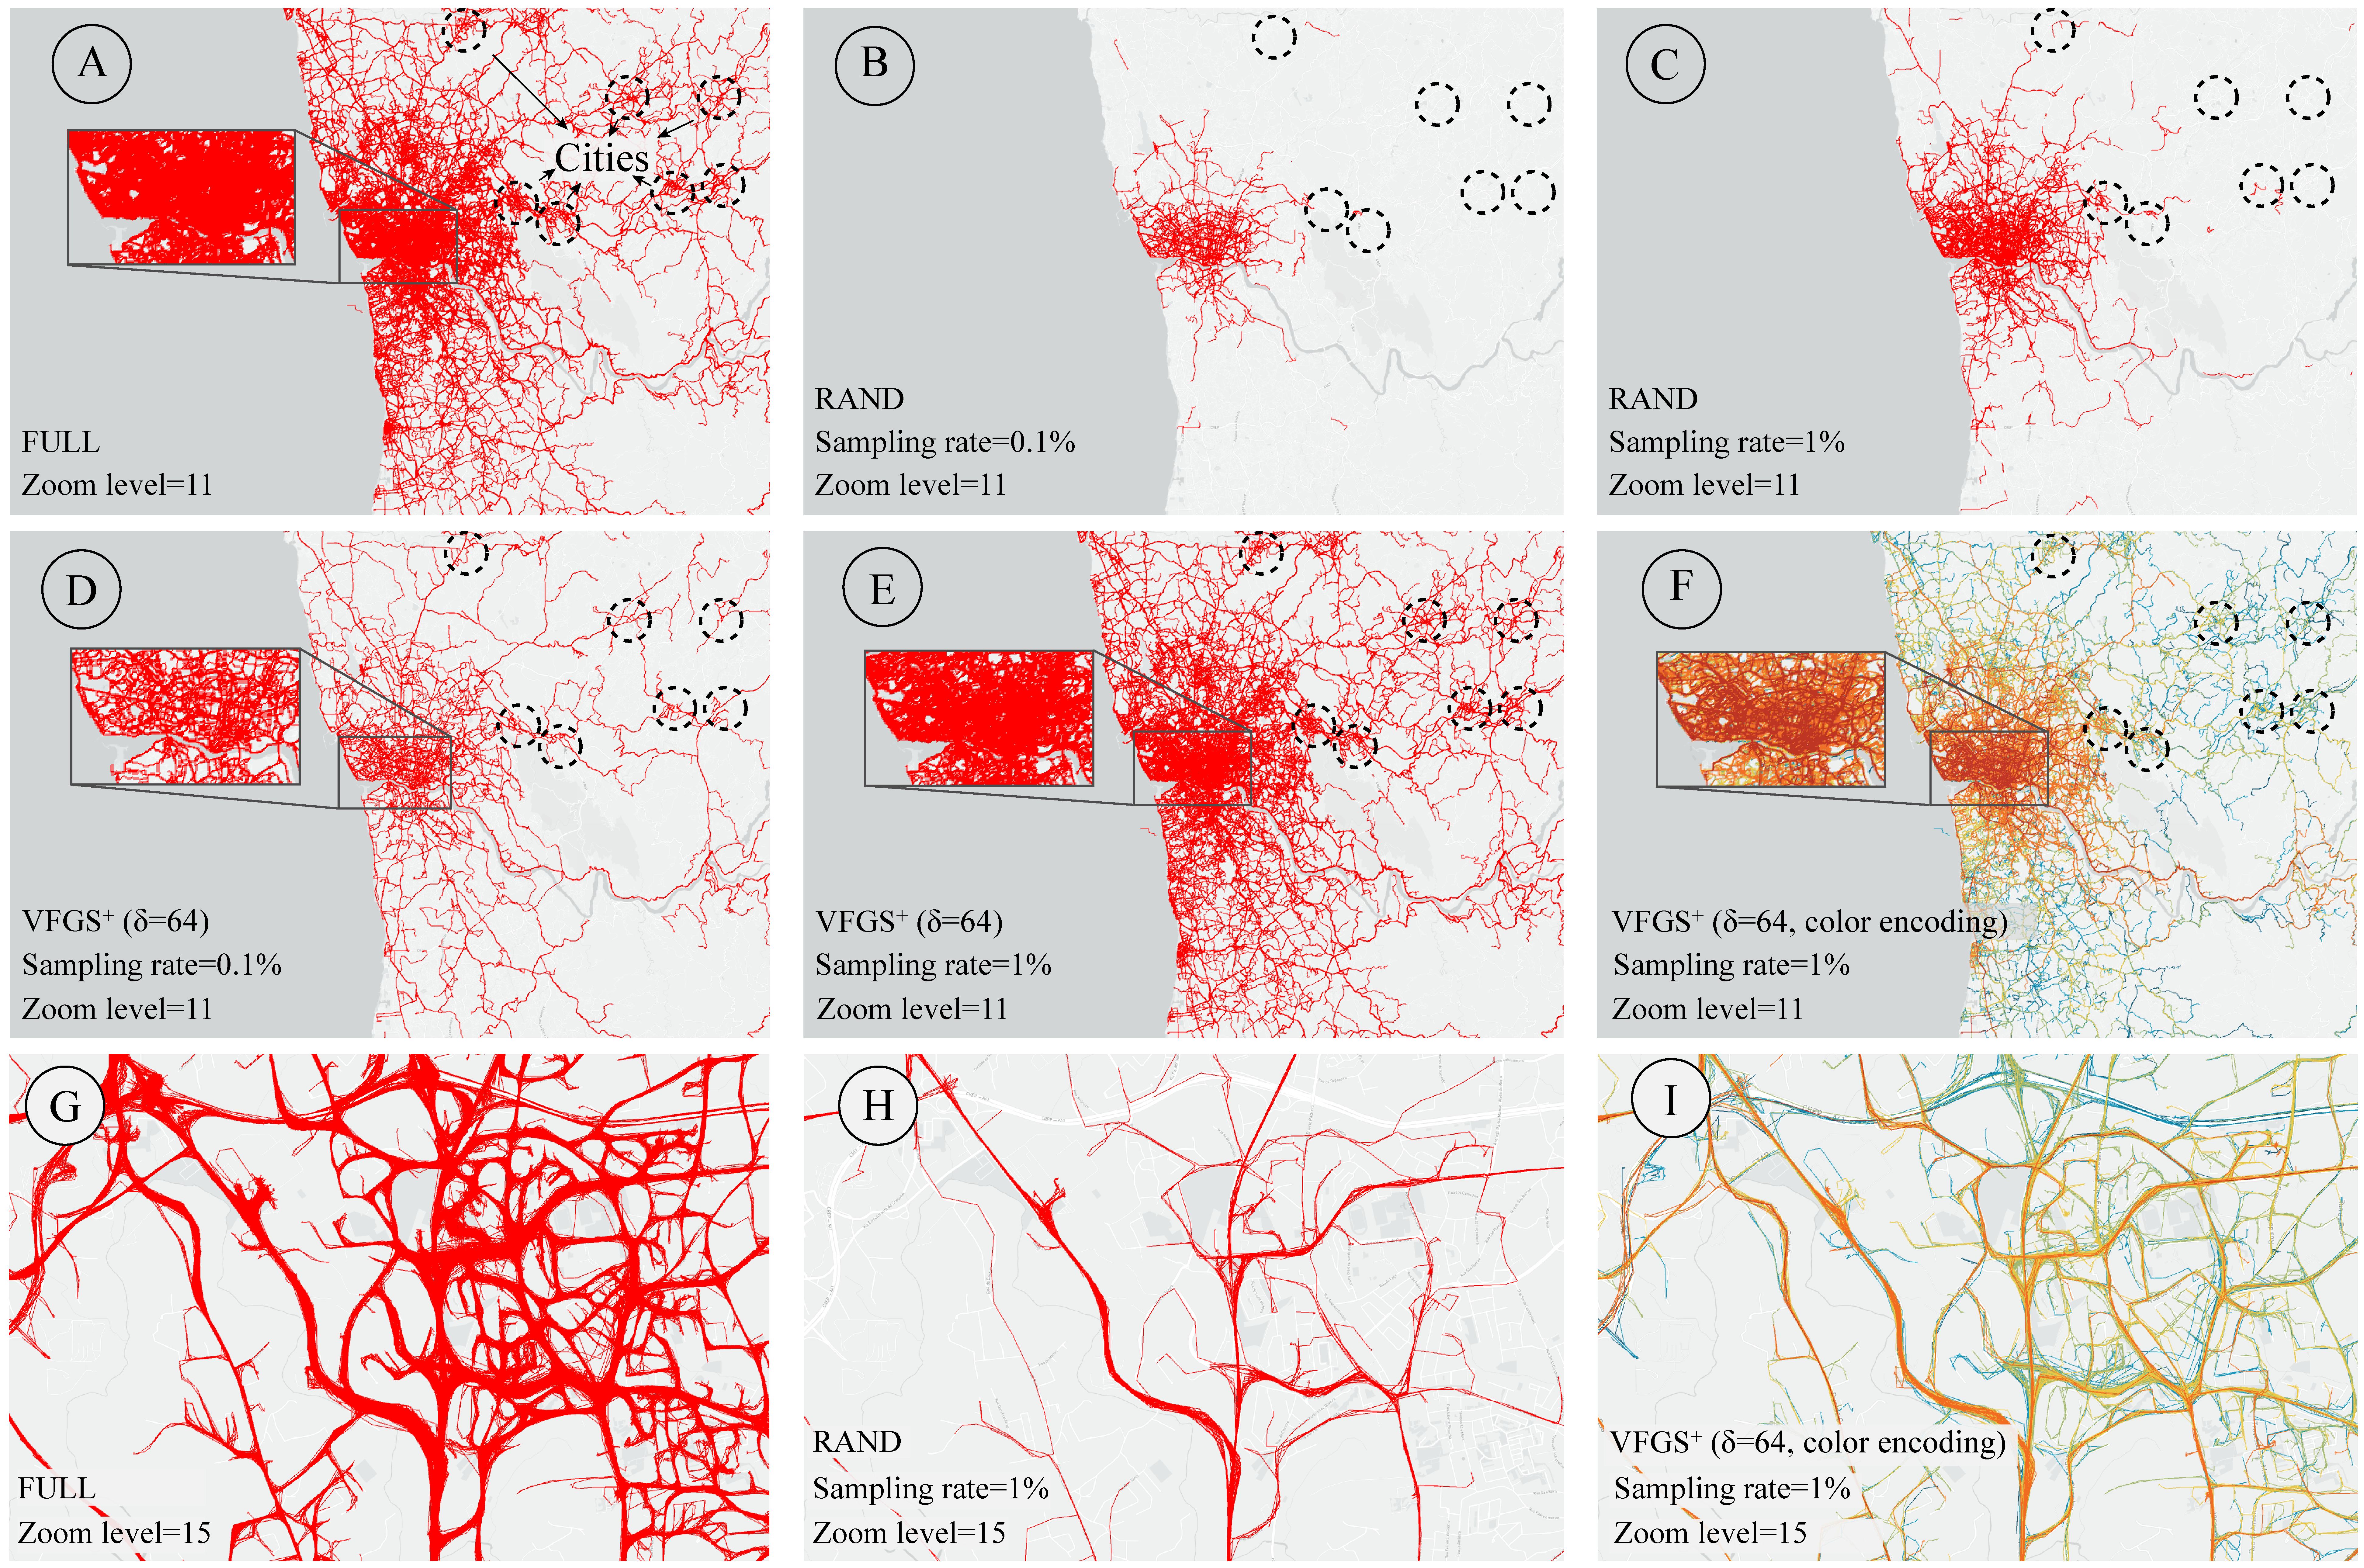
\includegraphics[width=0.82\textwidth]{pictures/Teaser.pdf}
	\vspace{-3mm}
	\caption{Visualization results comparison. (I) A is the visualization of the \pt{} taxi trajectory dataset at zoom level 11.
    B and C are visualizations of random sampling with sampling rate $0.1\%$ and $1\%$, respectively.
    D, E, F are visualizations of our proposed $\avats$ with different parameters.
    (II) G is visualization of the full \pt{} dataset at zoom level 15, where H and I are the corresponding visualized results of random sampling and $\avats$ (with sampling rate $1\%$), respectively.}
	\label{fig:teaser}
\trim 
\end{figure*}

{Sampling techniques are de-facto standards} for large-scale data analysis in both database and visualization communities.
In general, it samples a subset of data from the raw large-scale dataset, then it could be rendered efficiently by the graphics device.
For example, ScalaR~\cite{battle2013dynamic} employs a reduction layer between the visualization layer and the data management layer.
The reduction layer embedded a uniform random sampling algorithm to sample data randomly when the query results are large enough.
It then reduces the amount of data to be visualized.
However, the uniform random sampling method does not work well in the large trajectory data visualization problem as it does not have any guarantees about the sampling results.
Take Figure~\ref{fig:teaser}(B) and (C) as examples,
they are the visualization results of uniform random sampling method ($\rand$) on \pt{} taxi trajectory dataset with sampling rate $0.1\%$ and $1\%$, respectively.
Visually, both visualized results cannot capture the overview of the \pt{} trajectory dataset, as shown in Figure~\ref{fig:teaser}(A).

In database community,  Park et al. devised a visualization-aware sampling algorithm (VAS) for large-scale scatter points visualization  in~\cite{park2016visualization},
which offers theoretical quality guarantee on the visualization result.
However, the VAS techniques cannot be adapted to our problem as  (i) trajectory data is  more complex than scatter points (e.g., varying lengths, lack of compact representation),
and  (ii) the formulated visualization quality measure function in~\cite{park2016visualization} is only for scatter points, it cannot be used to measure the quality of trajectory visualization results.

In this work, we propose visual fidelity guaranteed sampling approaches for the line-based trajectory visualization problem.
The technical challenges of our proposals are
(i) how to define visual fidelity guarantee theoretically?
(ii) how to devise an efficient sampling algorithm which offers visual fidelity guarantee on the visualization result,
and (iii) how to overcome the visual clutter in large trajectory visualization.
Specifically, we first propose a novel pixel-based visual fidelity loss function between two visualization results formally.
With the visual fidelity loss function, we then prove it is NP-hardness to select a sized-$k$ subset of trajectories which has the minimal visual fidelity loss.
Next, we devise an approximate algorithm ($\vats$) which returns a sized-$k$ subset of trajectories and offers theoretical visual fidelity guarantee on the returning result.
Last, we address the visual clutter issue explicitly by taking data distribution and human perception capability into consideration in the advance approach ($\avats$).
Figure~\ref{fig:teaser}(D) and (E) show the visualization results of our proposal $\avats{}$ on \pt{} taxi trajectory dataset with {the} sampling rate $0.1\%$ and $1\%$, respectively.
Obviously, the visualization fidelity of them are much better than the uniform random sampling visualization results with the same sampling rates, see Figure~\ref{fig:teaser}(B) and (C).
Figure~\ref{fig:teaser}(F) is the returning result of our proposal which colors the trajectories {according to the trajectory representativeness}.
It has the same parameters of Figure~\ref{fig:teaser}(E).
Visually, the visual clutter in Figure~\ref{fig:teaser}(A) and (E) are alleviated in Figure~\ref{fig:teaser}(F).
In addition, our proposals are robustness with different zoom levels.
Figure~\ref{fig:teaser}(G), (H), and (I) depict the visualization results of the \pt{} dataset, the returning result of uniform random sampling $\rand$ and the returning result of $\avats$ with color encoding at zoom-level 15, for example, we can obtain them by zooming in the visualization result in Figure~\ref{fig:teaser}(A), (C), and (F), respectively.
Intuitively, the visualization result of our proposal $\avats$ in Figure~\ref{fig:teaser}(F) outperforms the uniform random sampling method $\rand$ in Figure~\ref{fig:teaser}(H) significantly.
It even performs better than Figure~\ref{fig:teaser}(G), the visualized result of the \pt{} dataset, as it reduces visual clutter in Figure~\ref{fig:teaser}(G) by using color encoding scheme to capture the representativeness of different trajectories.

The contributions of this paper are:
%\setlist{nolistsep}
%\begin{itemize}[noitemsep]
\squishlist
  \item We formulate the visual fidelity guaranteed sampling problem for large trajectory data visualization, and prove it is {NP-hard} in Section~\ref{sec:pro}.
  \item We devise an approximation algorithm $\vats$ with a suite of optimization techniques, e.g., submodularity, lazy computing, for it in Section~\ref{sec:sol}.
  \item We propose an advance approach $\avats$ to further enhance the effectiveness of our approximate algorithm, which {addresses} the visual clutter by introducing perception tolerance parameter,
  and encodes the representativeness of each {trajectory} by different colors in Section~\ref{sec:aa}.
  \item We conduct extensive experiments on real-world trajectory datasets to demonstrate the superiority of our proposals in Section~\ref{sec:exp}. Especially, we conduct comprehensive user studies to show {the} effectiveness on three real-world applications.
\squishend
%\end{itemize}

%Our proposal demonstrates their superiority over existing methods
%With the same sampling set size($1\%$), the proposed method generates a higher-fidelity visualization and .

%With the loss function, we analyze the hardness of the problem, and devise a visual quality guaranteed sampling algorithm for it.
%Figure~\ref{fig:compare} depicts an comparison among the ground truth,  uniform random sampling and our proposed method.
%With the same sampling set size($1\%$), the proposed method generates a higher-fidelity visualization and support the multi-resolution very well.
%At last, color encoding are applied to enhance the distribution of trajectories.

%


%\TB{Visualizing a large collection of trajectories are used frequently in map service or smart city applications.}
%The most popular and conventional method is the line-based visualization~\cite{chen2015survey}: connecting the passing points of movement objects by polylines.
%To handle the big dataset, many visualization products such as Spotfire~\footnote{\url{https://www.tibco.com/products/tibco-spotfire}}
%and Tableau~\footnote{\url{https://www.tableau.com/}} support advanced database management systems as a ``backend'' for the efficient data processing the query.
%The current visualization tools always don't scale well for the presentation of very large trajectory dataset due to the two challenges,
%visual clutter and limited rendering speed, which hinders the abilities of human-users for interactively exploring the dataset and identifying the movement patterns.
%In recent years, most of the visualization research works mainly try to address the visual clutter issue by proposing new techniques such as the
%spatial aggregation~\cite{zeng2013visualizing, von2015mobilitygraphs}, edge bundling~\cite{zeng2019route, thony2015vector} and density map~\cite{lampe2011interactive, scheepens2011interactive}.
%Instead, in this paper, we focus on the challenge of inefficient rendering in the large trajectory dataset by involving data sampling techniques.

%It is time consuming to generate very simple visualization when the data size become very large. Using Porto taxi data ~\footnote{\url{http://www.geolink.pt/ecmlpkdd2015-challenge/dataset.html}} as an example, Table~\ref{table:rendering_time} demonstrates the rendering time at each dataset size. \ZW{shall also mention which rendering toolkit is used here.} It shows that normal method takes more than 14 minutes (\ZW{seconds?}) to generate the graphics for 1 million trajectories, which is far beyond the human-acceptable response time for the interactive exploration~\cite{shneiderman1984response}.
%One work closely related to ours is ScalaR~\cite{battle2013dynamic}, which adds a reduction layer between visualization layer and data management layer. The reduction layer uses an uniform random sampling method to sample data once the query results are large enough, thus to reduce the amount of data to be visualized.
%Further more, Park et al. propose VAS~\cite{park2016visualization} which implements new sampling techniques to guarantee the visual quality.
%However, these sampling techniques are designed for the simple dataset, and have been approved effective in scatter plot or map plot.
%However, the trajectory sampling is more challenge due to the complexity of data form(e.g. varying lengths, lack of compact representation, difficulty in measuring the similarity) that makes traditional density-biased sampling techniques inappropriate.
%A naive solution to employ sampling idea for large-scale trajectory visualization problem is randomly selecting several trajectories from the data set then visualize it by graphics device.
%However, the visualization result may be not acceptable by the user because of the visual information loss in the sparse distributed regions.





%
%\begin{figure}[t]
%	\centering
%	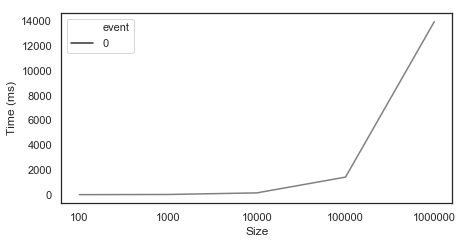
\includegraphics[width=0.4\textwidth]{pictures/introduction/timesize.png}
%	\vspace{-5mm}
%	\caption{The latency time for generating line-based visualization at each datasize.}
%	\vspace{-5mm}
%	\label{fig:rendering_time}
%\end{figure}




%The major challenges to design visual quality guaranteed sampling method are:
%(I) how to define visual quality theoretically? (II) how to guarantee the quality of the sampling-based visualization result?
%\TB{In this work, we study how to reduce the rendering time and preserve the visual quality for the large-scale trajectory visualization.}
%We extend the motivation of visualization-aware sampling to trajectory dataset and propose a novel sampling strategy, \textbf{v}isualization \textbf{a}ware \textbf{t}rajectory \textbf{s}ampling(VATS), that produces high-visual-quality line-based trajectory visualization at different zooming resolutions.
%%\QM{In this paper, we first proposed the visual fidelity loss function which effectively evaluates the visual loss of the sampling method. Then we minimize the loss function by transforming this problem to an optimization problem. Several solutions for efficiently solving the optimization problem are discussed.}
%We first format visual quality by defining the loss function between the visualization results of the whole dataset and sampled dataset.
%With the loss function, we analyze the hardness of the problem, and devise a visual quality guaranteed sampling algorithm for it.
%Figure~\ref{fig:compare} depicts an comparison among the ground truth,  uniform random sampling and our proposed method.
%With the same sampling set size($1\%$), the proposed method generates a higher-fidelity visualization and support the multi-resolution very well.
%At last, color encoding are applied to enhance the distribution of trajectories.
%
%\begin{figure}[t]
%	\centering
%	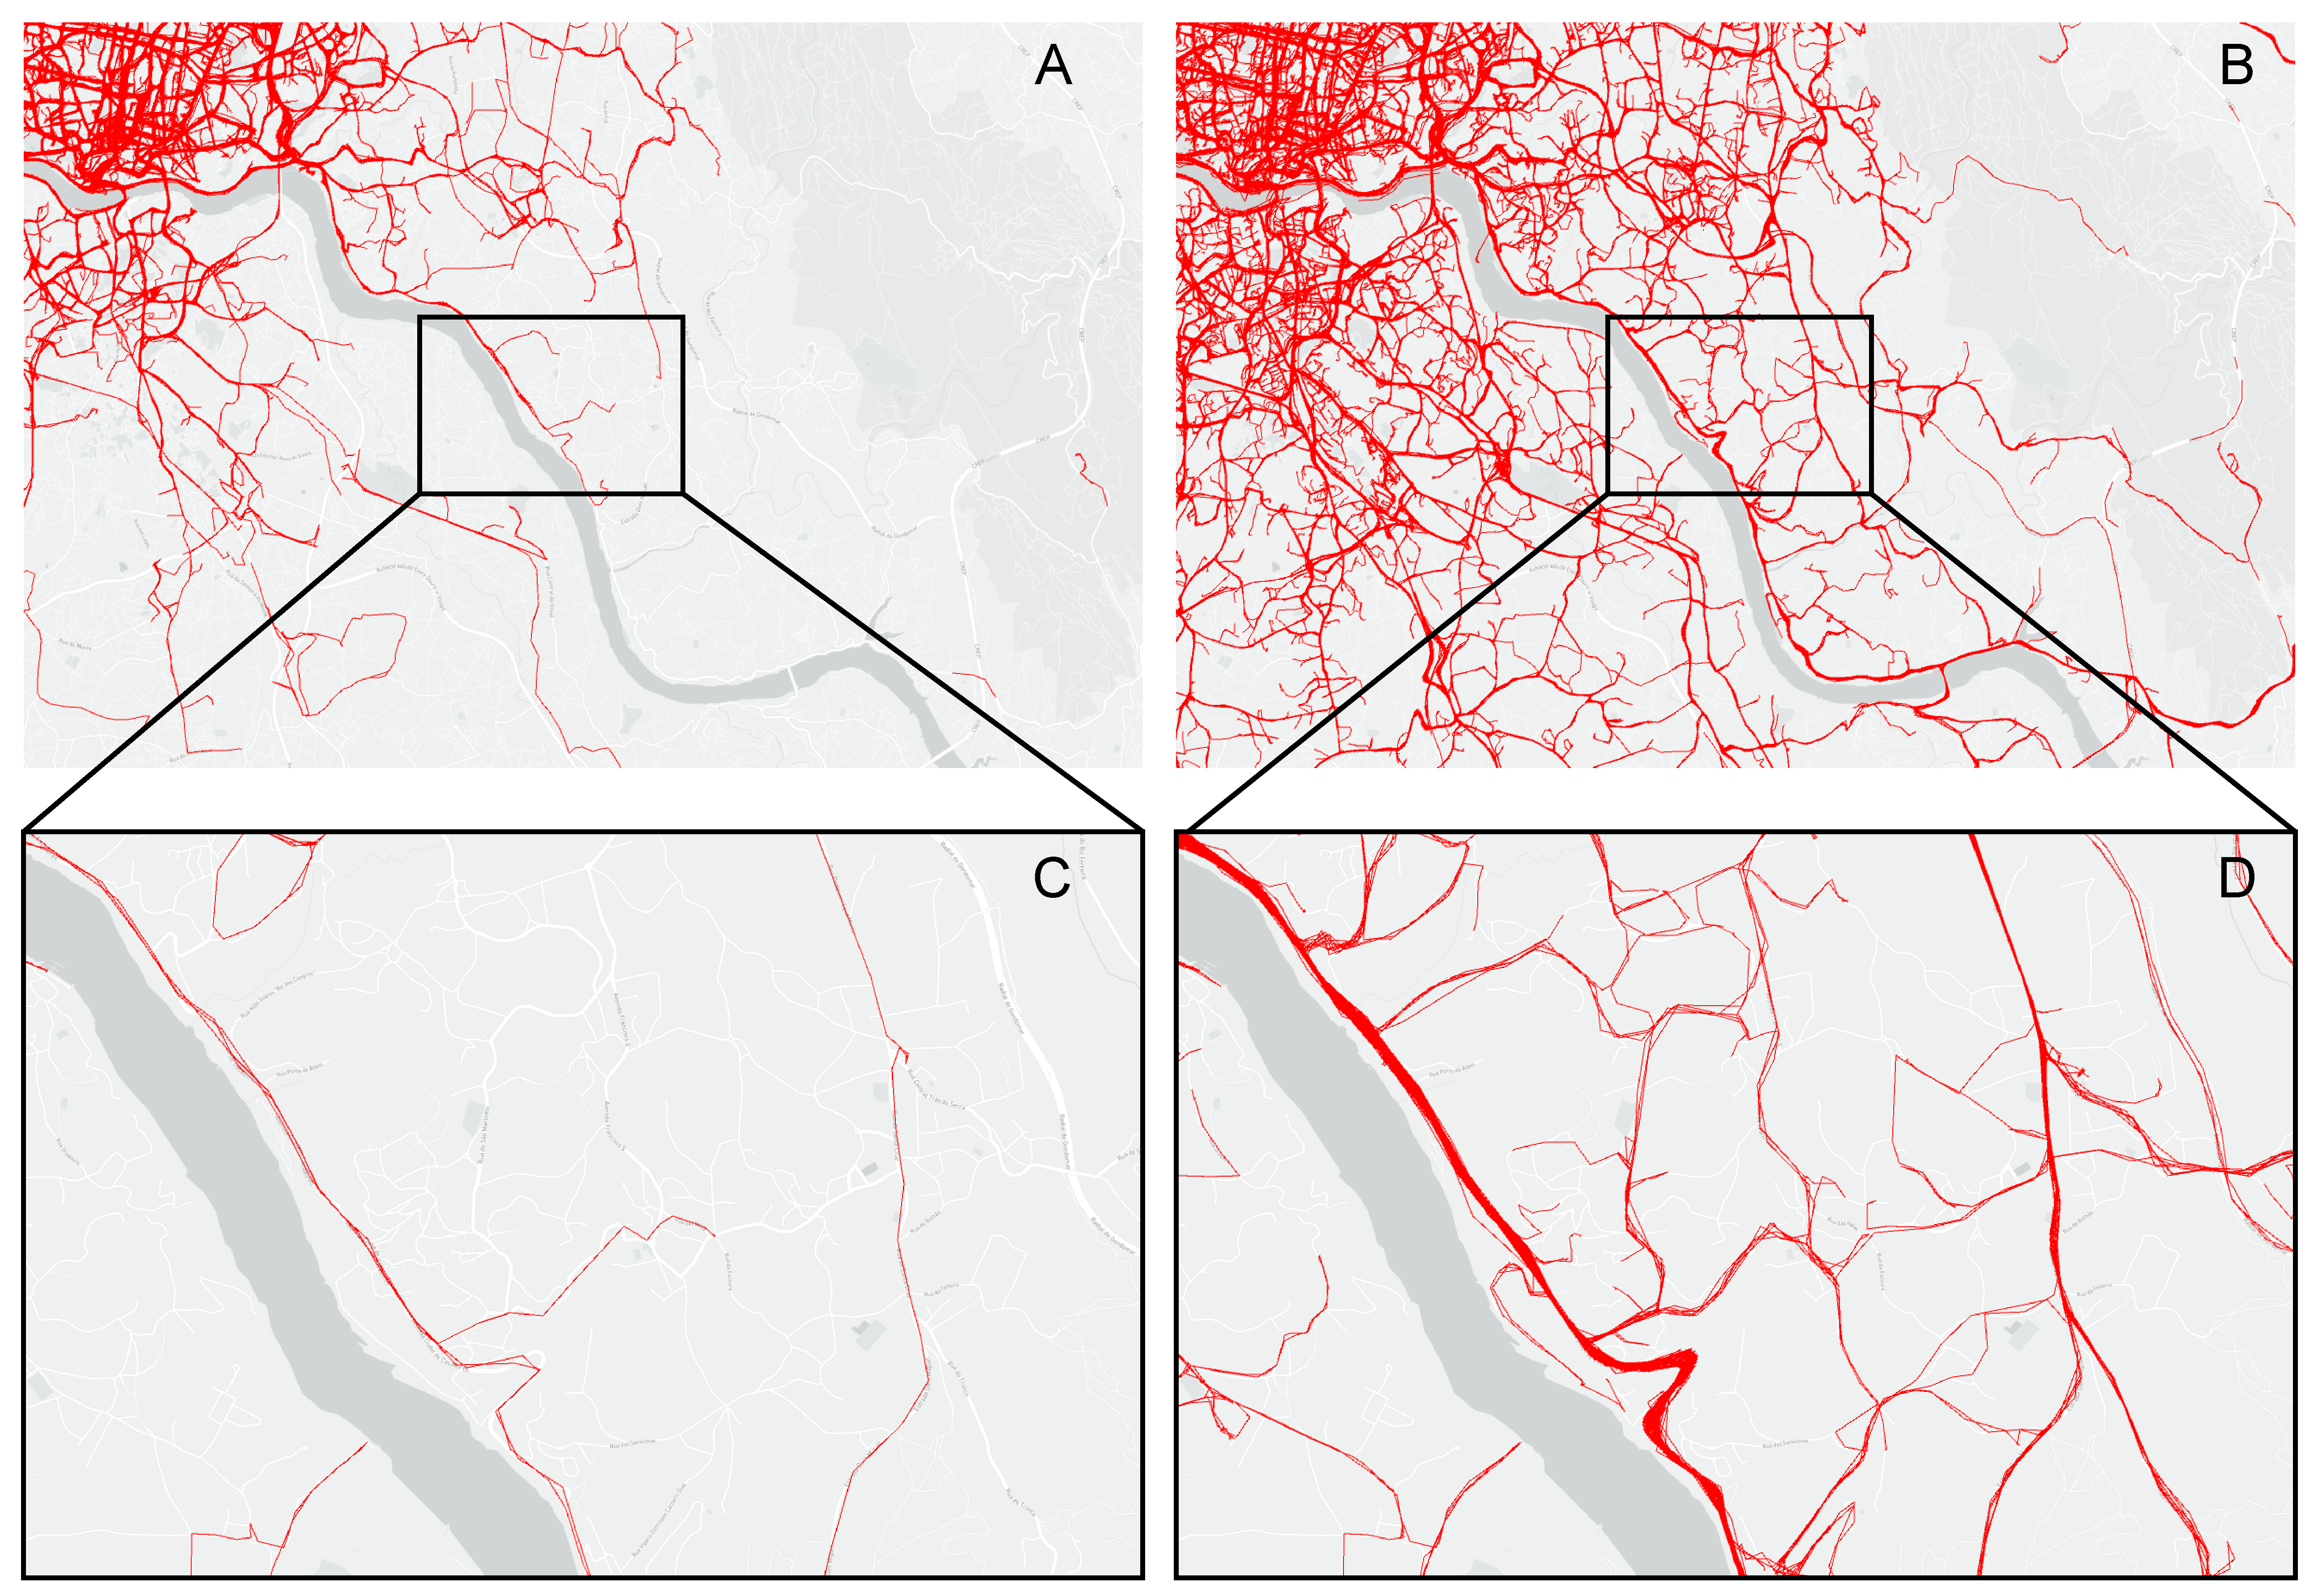
\includegraphics[width=0.44\textwidth]{pictures/introduction/effectiveness.pdf}
%	\vspace{-3mm}
%	\caption{Trajectory sampling generated by uniform random sampling(A,C) and VQGTS(B,D) at same sampling rate. In both high-level(A,B) and low level(C,D) view, our approach preserved more detail information about the trajectories especially for the sparse regions.}
%	\vspace{-5mm}
%	\label{fig:compare}
%\end{figure}
%

%
% \Bo{we can keep it at technical report.}
%The remainder of this paper is organized as follows.
%Section~\ref{sec:rel} discusses the related work.
%Section~\ref{sec:pro} formulates our problem and analyze its hardness.
%Section~\ref{sec:sol} provides an approximate solution for it, together with a suite of optimization techniques.
%Section~\ref{sec:aa} proposes an advanced solution for our problem.
%Section~\ref{sec:exp} elaborates our extensive experimental studies and our findings in detail.
%Section~\ref{sec:con} concludes this work and highlights the promising future directions.



\section{Related work}\label{sec:rel}
In this section, we survey previous work and focus on the most relevant pieces.
Section~\ref{sec:trajvisana} and ~\ref{sec:interactive} summarize the related works in trajectory visual analysis and interactive data visualization for large dataset, respectively.

\subsection{Trajectory Visual Analysis}\label{sec:trajvisana}
Trajectory is the most common representation of the object movements.
Each trajectory consists of a sequence of spatial locations (i.e., GPS points).
%To support the understanding and analyzing of the trajectory dataset,
%many visual analytical systems are proposed in the literature.
As stated in~\cite{chen2015survey}, existing trajectory visual analysis techniques can be classified into three categories according to visualization form,
i.e., point-based visualization, line-based visualization and region-based visualization.
We briefly introduce them and refer the interested readers to a recent survey~\cite{chen2015survey} for detail discussions.

The point-based visualization captures the spatial distribution overview of the GPS points in the moving object trajectories.
Many density-based methods, e.g., kernel density estimation, are applied in point-based visualization methods~\cite{liu2013vait,yang2016exploring,chae2014public,xie2008kernel, borruso2008network}.
%These point-based visualization methods reduce the visual clutter in large amount data by sacrificing the detail information of trajectories, e.g., the sequence order of GPS points.
%However, the point-based visualization result cannot identify the movement of the individual object and reveal the moving details~\cite{chen2015survey}, e.g.,  direction and path.
The region-based visualization approaches divide the whole region into sub-regions in advance, then visualize the aggregated information in each sub-region~\cite{guo2009flow,wood2010visualisation,von2015mobilitygraphs}.
These methods demonstrated their effectiveness to capture the macro-patterns.
In this work, we focus on the line-based visualization methods, which are widely used in visual analysis applications.
It uses polylines to show the trace of the object movements.
Through this, it preserves the continuous information of moving objects~\cite{guo2011tripvista,hurter2009fromdady}.
However, the line-based visualization methods suffer serious visual clutter due to the cross of the polylines in the large amount trajectories.
To alleviate this problem, several techniques have been proposed, such as the clustering-based techniques~\cite{ferreira2013vector, rinzivillo2008visually, von2015mobilitygraphs} and advanced interaction techniques~\cite{kruger2013trajectorylenses, ferreira2013visual}.
%In addition, the edge bundling techniques~\cite{zeng2019route,thony2015vector} are designed to reduce visual clutter.
%Specifically, they wrap up the similar trajectories into bundles, then generate clear visualization results.
Unlike existing line-based visualization techniques, we propose visual fidelity  guaranteed sampling approaches for line-based trajectory visualization with large-scale input data.
To the best of our knowledge, it is the first work which offers theoretical visual fidelity guarantee on the sampling result for large-scale line-based trajectory visualization.

\subsection{Interactive Visualization for Large Dataset}\label{sec:interactive}
{With the recent advancement of location-acquisition technology, the size of available trajectory dataset becomes extremely huge.}
For example, the operating taxis in Shenzhen generate {$\sim$}9.3GB trajectory data per day.
%Due to the limited rendering capability of modern commodity graphics device, generating visualizations for such scale of dataset takes considerable amount of time,
%or even impractical~\cite{park2016visualization}.
%In the literature, there are many works have been proposed to achieve interactive visualization {for} large dataset (not only trajectory dataset).
%We briefly elaborate the most representative pieces in subsequent section. %{(this subsection)}.
Figure~\ref{fig:framework} illustrates the architecture of interactive visualization systems for large datasets,
e.g., Spotfire~\cite{Spotfire}, Tableau~\cite{Tableau}, ATLAS~\cite{chan2008maintaining}, and Viate~\cite{yang2019vaite}.
{It} consists of three layers: the user interface in front-end, the optimization techniques in middle-layer, and the (cloud-based) database management system in the back-end.
{Typically, the researchers in visualization community focus on improving the effectiveness of data visualization at the front-end,
e.g., designing novel visualization methods to assist data analysts to obtain data insights effectively (D3~\cite{d3}).}
For the researchers in database community, they are working on the efficiency aspect for large data processing,
e.g., devising big data processing systems and techniques for efficient query processing at back-end (Spark~\cite{spark}).
In recent years, both visualization and database communities are dedicating to advance the techniques in interactive visual analysis for large-scale dataset,
e.g., the optimizations in the middle-layer (see Figure~\ref{fig:framework}).
We briefly elaborate these optimization techniques {in this section}. %as they are relevant to our technqiues in this work.


\begin{figure}
	\centering
	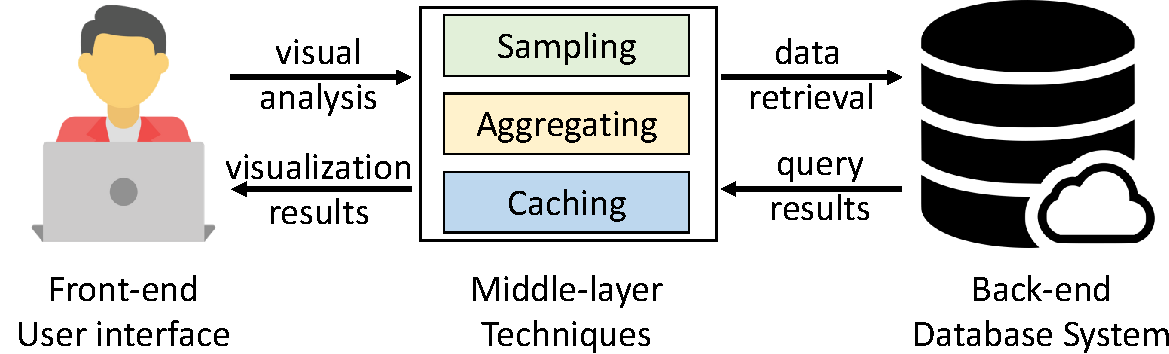
\includegraphics[width=0.40\textwidth]{pictures/framework/framework.pdf}
	\vspace{-3mm}
	\caption{Interactive visualization system architecture.} \label{fig:framework}
    \vspace{-6mm}
\end{figure}


\stitle{Aggregating-based techniques}
%{Aggregating-based techniques pre-process raw data with aggregation techniques (e.g., clustering) in the middle-layer, and yield fewer rendering objects for interactive visual analysis.}
%Returning to the trajectory visual analysis,
many works~\cite{wood2010visualisation,guo2009flow,von2015mobilitygraphs} divide the {spatial space} into basic units,
then visualize the information upon them by aggregation algorithms for trajectory visual analysis tasks.
For more details of other aggregating-based techniques, we refer the reader to the related works~\cite{andrienko2008spatio,adrienko2010spatial}.
%However, aggregating-based methods will cause information loss definitely.
%For instance, the continuous spatial traces of the moving objects are always missing and the rarely appeared trajectories are easily to be ignored.
Our problem and solutions are different from these research works as we focus on visualizing the raw input data, instead of the aggregated results.

\stitle{Sampling-based techniques}
Sampling techniques are widely used in both visualization and database communities ~\cite{battle2013dynamic,chen2014visual,park2016visualization}.
%are well-studied in the interactive visualization problems with large-scale input data.
%It is 
%In particular, ~\cite{chen2014visual} devised a sampling algorithm to preserve the meaningful data items. 
% according to the analyzing requirement such as the multi-class data analysis and hierarchical exploration.
The most relevant work of ours in the literature is~\cite{park2016visualization}, which designed for the scatter plot and aim to not only solve the overdrawing of the points but also try to preserve the information distribution of the original dataset.
%Specifically, they formulated a loss function which evaluates the visual loss of the sampling result effectively,
%they validate the proposed method by three common visualization tasks, e.g., regression, density estimation and clustering.
However, the techniques in~\cite{park2016visualization} cannot be adapted to our large-scale trajectory visualization problem
as trajectory data is more complex than scatter points.

%(i) the complexity of the trajectories~\cite{pelekis2010unsupervised}, and (ii) the loss function and its corresponding solutions are specified for scatter plot, not applicable for line-based trajectory visualization.
%For trajectory visual analysis,  most of the existing trajectory sampling techniques (if not all) cluster the trajectories at first,
%then select the most representative trajectories from each cluster and visualize them.
%It is impractical to provide interactive visualizations for real-world applications as
%trajectory clustering is still an open problem in both database and visualization communities~\cite{panagiotakis2011segmentation,agarwal2018subtrajectory}.

%as
%(i) the trajectory similarity computation and clustering algorithms are very expensive~\cite{pelekis2007similarity},
%and (ii) the 
Unlike the above research works, in this paper, we propose visual fidelity guaranteed sampling approaches for the large-scale trajectory visualization problem,
we demonstrate the superiority of our proposals by case-, user- and qualitative studies in real world datasets.


\stitle{Caching-based and other techniques}
%Caching is commonly used to improve the performance of large data processing system, e.g., search engine~\cite{xu2015diversified}.
Chan et al. present ATLAS~\cite{chan2008maintaining} which utilizes caching techniques for the efficient data communication between server and client.
In addition, it also exploits the powerful multi-core server to accelerate visual analysis task processing from the middle-layer to the back-end.
Piringer et al.~\cite{piringer2009multi} propose a multi-threading architecture for the interactive visual exploration,
which utilizes multi-core devices and avoids the multi-threading pitfalls to provide quick visual feedback.
{Our} proposed techniques in this work are orthogonal to the researches in this category.



%Current advancing sampling techniques in the visualization domain are mostly
%Some works design advanced sampling algorithms to preserve the meaningful data items according to the analyzing requirement such as the multi-class data analysis and hierarchical exploration~\cite{chen2014visual}. Furthermore, to the usage of more visual channels of the points other than location such as color~\cite{chen2014visual}, size~\cite{woodruff1998constant} and opacity are discussed.
%Closely related to our work, Park et al.~\cite{park2016visualization} proposed the visualization-aware techniques for the scatter plot.
%
%In comparison with the sampling techniques for scatter plot, the trajectory sampling is more challenging because of the complexity of the trajectories~\cite{pelekis2010unsupervised}.
%
%
%Many exiting visual analytics systems leverage powerful database manage system as the backend to facilitate the fast data processing. Based on the solution proposed in ScalaR~\cite{battle2013dynamic}, a common visualization framework involving sampling technique is illustrated as Figure~\ref{fig:framework}, where a sampling layer is set between the backend and frontend. Since the sampling methods are always designed for complicated task, the algorithms may not be efficient enough to support the interactive data exploration. Thus the cache model is always implemented to save the sampling results. In our scenario, the users query large amount of data(e.g. all Shenzhen trajectories in one week) once and then conduct interactive multi-resolution exploration based on the sampled data, thus the method need to guarantee the visual quality well across different resolutions.
%
%Sampling is a delta-facto solution for the problems with big data. Target at the sampling requirement, the naive solutions such as uniform random sampling cannot generate acceptable because the serious visual information loss. In this section, we first define a loss function to evaluate the visual quality between the visualization results between whole dataset and sampled subset. Then we analyze the hardness of the problem and design algorithms for it.
%
%
%\begin{figure}[t]
%	\centering
%	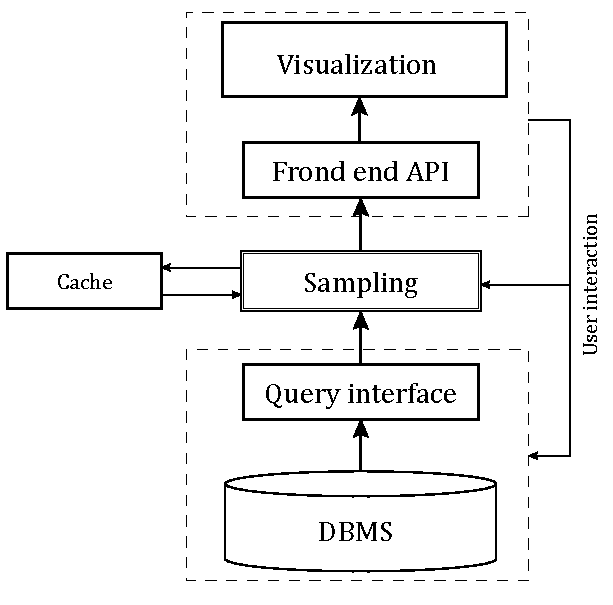
\includegraphics[width=0.3\textwidth]{pictures/framework/DBVAframework.pdf}
%	\vspace{-5mm}
%	\caption{A visualization framework involving sampling layer between the front-end and database management system.}
%	\vspace{-5mm}
%	\label{fig:framework}
%\end{figure}
%


\section{Problem Statement}\label{sec:pro}
In this section, we first define our research problem in Section~\ref{sec:def} formally.
Section~\ref{sec:hard} analyzes the hardness of our research problem.

\subsection{Problem Definition}\label{sec:def}
As we analyzed in Section~\ref{sec:intro}, the large-scale (e.g., hundreds of millions GPS points) line-based trajectory visualization problem is very challenging due to the large data size and limited rendering capability of graphics devices.
To make matters worse, the visualization result of large-scale trajectory dataset suffers visual clutter seriously.
In this work, we focus on how to visualize large-scale trajectory dataset efficiently and effectively.
In particular, our objective is to devise a visual fidelity guaranteed sampling method for large trajectory data visualization.
The major challenges to achieve this goal are:
(i) how to define visual fidelity theoretically? (ii) how to guarantee the visual fidelity of the sampling-based visualization result?
We commence our presentation by defining our research problem formally as follows.

\begin{problem}[Large-scale trajectory visualization problem]\label{prob:def}
Given a large-scale trajectory dataset $\D$ and a sampling rate $\alpha$,
the trajectory visualization problem is selecting a subset of trajectories $\oR \subseteq \D$ with $|\oR| \leq \alpha |\D|$,
such that visual fidelity loss function $loss(\oR,\D)$ is minimized.
\end{problem}

%From the user’s perspective, there are many ways to define the loss function $loss$ between the visualization result qualities of the sampled subset $\oR$ and the whole dataset $\D$.
%For example, \cite{park2016visualization} defined point-based loss function for very large scatter points visualization.
%However, it is not applicable for trajectory data visualization.
%In order to address that, we propose an novel loss function for trajectory visualization problem.


The key to solving the large-scale trajectory visualization problem (see Problem~\ref{prob:def}) is defining the visual fidelity loss function properly.
Intuitively, the visual fidelity of the sampled visualization results $\oR$ w.r.t. the original dataset $\D$ depends on the user specified visualization level of details (a.k.a., LOD).
Given an empty canvas (e.g., displaying device) with a user specified level of details,
the visualization process is rendering the trajectories into canvas with the given level of details, e.g., the number of pixels in each row and each column.
Considering a trajectory data set $\D$ and a subset of trajectories $\oR \subseteq \D$,
the visual fidelity loss between $\oR$ and $\D$ is defining as the different pixels of the visualization results about $\oR$ and $\D$ in the canvas with specified LOD.
We then define the visual fidelity loss function of sampling-based trajectory visualization problem as $loss(\D, \oR) = \frac{|\V(\D) - \V(\oR)|}{|\V(\D)|}$,
where $\V()$ measures the rendered pixels in the canvas of the input trajectory dataset.

Therefore, given a trajectory data set $\D$ and a sampling rate $\alpha$,
our research objective is finding subset $\oR$, such that  the visualization fidelity loss function $loss(\D, \oR)$ is minimized:
$$ \min_{\oR \subseteq \D, |\oR| \leq \alpha |\D|}  loss(\D, \oR) =  \frac{|\V(\D) - \V(\oR)|}{|\V(\D)|}. $$ %\\ %\nonumber


%  \Leftrightarrow  & \min_{\oR \subseteq \D, |\oR| = k}  \V(\D) - \V(\oR) \\ \nonumber
%  \Leftrightarrow  & \min_{\oR \subseteq \D, |\oR| = k}  \sum_{\forall \D_i \in \D} \V(\D_i) - \V(\oR)
%Intuitively, the visualization quality from user's perspective highly depends on the resolution of displaying device,
%e.g., the number of distinct pixels in each dimension that can be displayed.

%Given a high resolution displaying device, data objects set $\D$, and a subset of data objects $\oR \subseteq \D$.
%The visualization quality loss between $\oR$ and $\D$ is defining as the different pixels of the visualization results of $\oR$ and $\D$ in the given display device.
%Given a trajectory data set $\D$ and an integer $k$,  our research objective is selecting a sized-$k$ subset of trajectories which minimize
%the visualization quality loss function $loss(\D, \oR)$.
%Formally, the loss function is defined as $loss(\D, \oR) = \V(\D) - \V(\oR)$.



\subsection{Hardness Analysis}\label{sec:hard}
For the sake of presentation, we analyze the hardness of our research objective with a simple render manner of visualization result.
We are aware there exist complex rendering schemes, e.g., different pixels has different colors, we will consider them shortly.
In particular, for each pixel in the canvas with simple render manner, it will be rendered if there is a trajectory pass through it, otherwise it will not be rendered.
Suppose each pixel in the canvas has an unique id, let $\MU$ be the universal set of all pixels in the canvas.
For each trajectory $t_i \in \D$, it consists of a set of pixels in the canvas.
In other words, the pixel set of each trajectory $t_i \in \D$ is a subset of $\MU$.
Consequently, the pixel set of the selected trajectory set $\oR$ is also a subset of $\MU$ as $\oR = \cup_{t_i \in \oR} t_i$.


Our research objective is minimizing loss function $loss(\D, \oR) =  \frac{|\V(\D) - \V(\oR)|}{|\V(\D)|}$ subject to $\oR \subseteq \D$ and $|\oR| \leq \alpha |\D|$.
Given an empty canvas, the visualized/rendered pixels of the input trajectory dataset $\D$ is a constant set, denotes as $\mathsf{C}$.

Hence, our research objective of Problem~\ref{prob:def} can be transformed as follows:
\begin{align}\label{eqn:obj2} \nonumber
\text{Objective}: & \min_{\oR \subseteq \D, |\oR| = \alpha |\D|}  \frac{|\V(\D) - \V(\oR)|}{|\V(\D)|} \Leftrightarrow \min_{\oR \subseteq \D, |\oR| = \alpha |\D|}  \frac{|\mathsf{C} - \V(\oR)|}{|\mathsf{C}|}  \\ \nonumber %
& \Leftrightarrow \min_{\oR \subseteq \D, |\oR| = \alpha |\D|}   - |\V(\oR)| \Leftrightarrow \max_{\oR \subseteq \D, |\oR| = \alpha |\D|}  |\V(\oR)|  \\ \nonumber
& \Leftrightarrow \max_{\oR \subseteq \D, |\oR| = \alpha |\D|} | \cup_{t_i \in \oR} t_i |
\end{align}

It is equivalent to the well-known set cover maximization problem.
Specifically, given an integer $k = \alpha |\D|$, and a collection trajectory pixel set $\D = \{t_1, t_2, \cdots, t_n \}$ with $\forall t_i \subset \MU$,
the objective of the set cover maximization problem is finding a subset $\oR \subset \D$ such that $|\oR| \leq k$ and the number of covered pixels in $|\cup_{t_i \in \oR} t_i|$ is maximized.
We omit the proof of its NP-hardness, as it has been shown in~\cite{setcover}.


%It is equivalent to select sized-$k$ trajectory set $\oR$ from $\D$ which $\cup_{\oR_i \in \oR} \oR_i$ is maximized.
%It is a NP-hard problem as we proved in Lemma~\ref{lem:np}.

%\begin{lemma}[NP hard]~\label{lem:np}
%Given a trajectory dataset $\D$ and an integer $k$,
%The sampling-based trajectory visualization problem (see Problem~\ref{prob:def}) is NP-hard.
%\end{lemma}

%We omit the proof of Lemma~\ref{lem:np} as it is a typical set cover maximization problem\footnote{\url{https://en.wikipedia.org/wiki/Maximum_coverage_problem}}, which is a well-known NP-hard problem in literature.



%\section{Visual Fidelity Guaranteed Sampling Approach}\label{sec:sol}
\section{Our Solution: $\vats$}\label{sec:sol}
Due to the hardness of the Problem~\ref{prob:def}, we first introduce a straight-forward solution, i.e., uniform random sampling $\rand$.
Specifically, it randomly selects $k$ trajectories from dataset $\D$ and stores them in result set $\oR$.
Last, we render these selected trajectories in $\oR$ as the visualization result.
Obviously, the uniform random sampling $\rand$ algorithm does not provide any guarantee on the visual fidelity of the sampled result set.

In this section, we next propose a visual fidelity guaranteed sampling method $\vats$ in Section~\ref{sec:greedy}.
Last, we devise several optimizations to improve the efficiency of our proposal $\vats$ in Section~\ref{sec:opt}.





\subsection{Visual Fidelity Guaranteed Sampling}\label{sec:greedy}
In this section, we present our visual fidelity guaranteed sampling algorithm for Problem~\ref{prob:def}.
We first elaborate the correlation between visual fidelity of sampled set $\oR$ and user zoom level.
For a given result sampled set $\oR \subseteq \D$, it has different visual fidelity loss values at different user zoom levels.
The reason is the resolutions of $\oR$'s visualized result are different at different zoom levels.
For example, Google map~\cite{googlemap} provides zoom levels range from 0 to 20,
where level 0 is the lowest level (e.g., the whole world), level 20 is the highest level (e.g., individual building, if available).
In order to devise a zoom level oblivious visualization for sampled dataset $\oR$,
we use the highest zoom level to define the size of each pixel in the canvas in our problem.
It means for each trajectory $t_i \in \D$, it is a set of pixels in the canvas at the highest zoom level.

With the above setting, we next describe our visual fidelity guaranteed sampling algorithm in Algorithm~\ref{alg:greedy}, which employs greedy paradigm.
In particular, it finds the trajectory $tmp$ in $\D$ which maximize the result set of $|\oR \cup tmp|$ at each iteration, as Line~\ref{line:max} shown in Algorithm~\ref{alg:greedy}.
It terminates after $k=\alpha |\D|$ iterations and returns $\oR$ as result set for rendering.

\vspace{-2mm}
\begin{algorithm}
    \caption{$\vats(\D,k=\alpha |\D|)$} \label{alg:greedy}
    \begin{algorithmic}[1]
    \State Initialize result set $\oR \leftarrow \emptyset$
    \While{$|\oR| < k$}
        \State $tmp \leftarrow argmax_{t_i \in \D} |\oR \cup t_i|$ \label{line:max}
        \State $\oR \leftarrow \oR \cup \{ tmp \}$
    \EndWhile
    \State Return $\oR$
    \end{algorithmic}
\end{algorithm}
\vspace{-2mm}

Interestingly, Algorithm~\ref{alg:greedy} offers theoretical visual fidelity guarantee of the returning result $\oR$, as proved in Theorem~\ref{the:ratio}~\footnote{We omitted all the proofs of the theorems and lemmata in this work due to space reasons, and refer the interested readers to our technical report\cite{techreport}.}.

\begin{theorem}~\label{the:ratio}
Algorithm~\ref{alg:greedy} provides $1-(1-1/k)^k \geq (1-1/e) \approx 0.632$ approximation result for large-scale trajectory visualization problem (i.e., Problem~\ref{prob:def}).
\end{theorem}

%\begin{proof}
%The optimal solution of Problem~\ref{prob:def} covers $OPT$ pixels in $k$ iterations.
%Let $a_i$ be the number of newly covered pixels at the $i$-th iteration, $b_i$ is the total number of covered pixels up to the $i$-th iteration (i.e., $b_i = \sum_{j=1}^{i}a_i$),
%and $c_i$ be the uncovered pixels after $i$-th iteration (i.e., $c_i = OPT-b_i$).
%According to greedy paradigm, we can conclude the number of newly covered pixels at the $(i+1)$-th iteration is always greater than or equal to $\frac{1}{k}$ of the number of uncovered pixels after the $i$-th iteration, i.e., $a_{i+1} \geq \frac{c_i}{k}$.
%We prove Theorem~\ref{the:ratio} by proving $c_{i+1} \leq (1-1/k)^{i+1} \cdot OPT$.
%It holds $c_1 \leq (1-1/k) \cdot OPT$ as follows.
%\begin{align} \nonumber
%& a_1 \geq c_0 \cdot 1/k = 1/k \cdot OPT \text{~~~as we concluded~~~} a_{i+1} \geq \frac{c_i}{k}\\ \nonumber
% \Leftrightarrow  & b_1 \geq 1/k \cdot OPT  \Leftrightarrow  -b_1 \leq - 1/k \cdot OPT  \text{~~~as~~~} a_1 = b_1\\ \nonumber
% \Leftrightarrow & OPT - b_ 1 \leq OPT - 1/k \cdot OPT  \Leftrightarrow  c_1 \leq (1-1/k) \cdot OPT
%\end{align}
%For inductive hypothesis assume $c_{i} \leq (1-1/k)^i \cdot OPT$. Thus,
%\begin{align} \nonumber
%& c_{i+1} = c_i - a_{i+1} \leq c_i - c_i/k = (1-1/k) \cdot c_i = (1-1/k)^{i+1} \cdot OPT
%\end{align}
%
%Hence, it holds $c_k \leq (1-1/k)^{k} \cdot OPT$.
%It is equivalent to $b_k \geq (1 - (1-1/k)^{k}) \cdot OPT \geq (1-1/e) \cdot OPT \approx 0.632 \cdot OPT$.
%\end{proof}


\subsection{Optimization Techniques}\label{sec:opt}
With the above analysis, Algorithm~\ref{alg:greedy} ($\vats$) provides a visual fidelity guaranteed sampling algorithm for large-scale trajectory data visualization problem.
However, it is inefficient for (very) large trajectory dataset (e.g., millions of trajectories) as the time complexity analyzed in the following Lemma~\ref{lem:cost}.

\begin{lemma}[Time Complexity]~\label{lem:cost}
Given trajectory dataset $\D$ and an integer $k = \alpha |\D|$, the time complexity of Algorithm~\ref{alg:greedy} is $O(\alpha \cdot m \cdot |\D|^2)$, where $m$ is the maximum length of all trajectories in dataset $\D$.
\end{lemma}

%\begin{proof}
%At each iteration ($k = \alpha |\D|$ iterations in total),
%it computes the uncovered pixels of each trajectory in dataset $\D$ with $O(m)$ cost.
%The dataset $\D$ has $O(|D|)$ trajectories.
%Thus, the total cost is $O(k \cdot m \cdot |\D|)=O(\alpha \cdot m \cdot |\D|^2)$.
%\end{proof}

\stitle{Example} Given \pt{} trajectory dataset, it has 2.39 millions of taxi trajectories, the maximum length in it is 3,490.
It takes 413.6 seconds to return a subset $\oR$ with sampling rate $0.1\%$.
Obviously, it is impractical for interactive trajectory explorations.

Due to the inefficient of our visual fidelity guaranteed sampling approach in Algorithm~\ref{alg:greedy},
we then devise performance optimizations to accelerate its running time.
The core idea is utilizing the submodularity of the covered pixels of result set $\oR$, as shown in Lemma~\ref{lem:submodular}.

\begin{lemma}[Submodularity]\label{lem:submodular}
Suppose the contribution of trajectory $t$ to the result set $\oR$ is $\Delta(\oR, t) = |\oR \cup t| - |\oR|$.
Given a trajectory $t$ and two result sets $\oR,\oR^{'}$, where $\oR \subset \oR^{'}$ and $t \notin \oR$,
it holds $ \Delta(\oR, t) \geq \Delta(\oR^{'}, t)$.
\end{lemma}

%\begin{proof}
%The contribution value of trajectory $t$ to a given result set $\oR$ (e.g., $\Delta(\oR, t) = |\oR \cup t| - |\oR|$) is the new covered pixels of $t$ w.r.t. result set $\oR$, i.e., $|t| - |\oR \cap t|$.
%It holds $t \cap \oR \subseteq  t \cap \oR^{'}$ as $\oR^{'}$ is a superset of $\oR$.
%Thus, we have $|t| - |t \cap \oR| \geq |t| - |t \cap \oR^{'}|$.
%Hence, it holds $\Delta(\oR, t) = |\oR \cup t| - |\oR| \geq |\oR^{'} \cup t| - |\oR^{'}|= \Delta(\oR^{'}, t)$.
%\end{proof}

\begin{figure}
 \centering
 \small
 \begin{tabular}{cc}
   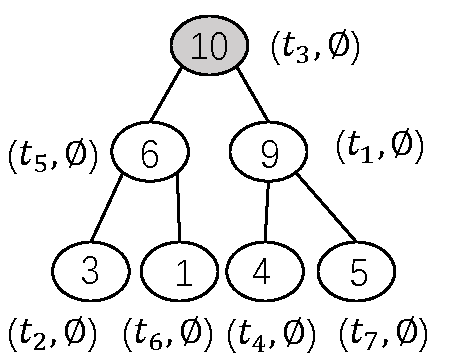
\includegraphics[width=0.35\columnwidth]{pictures/1st}
   &
   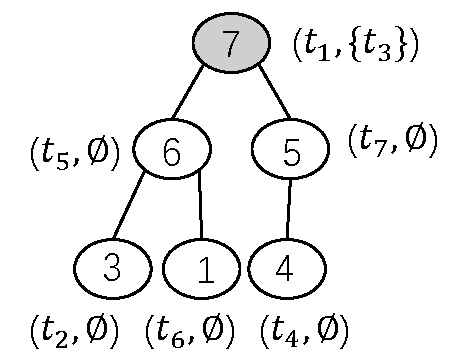
\includegraphics[width=0.35\columnwidth]{pictures/2nd}
   \\
   A) 1st iteration
   &
   B) 2nd iteration
 \end{tabular}
 \vspace{-3mm}
 \caption{Lazy computing manner.} \label{fig:heap} %via the submodularity in Lemma~\ref{lem:submodular}
 \vspace{-6mm}
\end{figure}


With the help of submodularity in Lemma~\ref{lem:submodular}, it reduces many unnecessary trajectory contribution value computations.
In particular, we maintain a max-heap for the number of uncovered pixels of each trajectory,
we employ a lazy computing manner, i.e., only compute the contributions of a given trajectory when it is necessary.
Figure~\ref{fig:heap}(a) shows a tiny max-heap example about the numbers of uncovered pixels of each trajectory from $t_1$ to $t_7$ with result set $\oR=\emptyset$.
At the 1st iteration, the root node of the max-heap will be selected, i.e., $t_3$ in Figure~\ref{fig:heap}(A).
At the 2nd iteration, the number of uncovered pixels of the root node $t_1$ is updated to 7 w.r.t. result set $\oR = \{t_3 \}$ (see gray node at Figure~\ref{fig:heap}(B)).
Then $t_1$ will be selected at the 2nd iteration without computing the number of uncovered pixels in other trajectories, i.e., all white nodes at Figure~\ref{fig:heap}(B).
The reason is the contribution of the trajectories in all white nodes will be less than 7 according to the submodularity in Lemma~\ref{lem:submodular}.

%In summary, the number of uncovered pixels in each trajectory will only be computed with the latest result set $\oR$ when it is necessary in the lazy computing manner,
%e.g., only $t_1$ will be updated at the 2nd iteration in Figure~\ref{fig:heap}.
%It reduces many unnecessary computations through the lazy updating manner, e.g., all white nodes did not update at the 2nd iteration in the above example.

%We then analyze the time complexity of Algorithm~\ref{alg:greedy} with lazy computing manner in Theorem~\ref{lem:lazy}.
%
%\begin{lemma}[Optimized Time Complexity]~\label{lem:lazy}
%Given trajectory dataset $\D$ and an integer $k= \alpha |\D|$, the time complexity of Algorithm~\ref{alg:greedy} with lazy computing manner is $O(\alpha \cdot m \cdot x |\D| \log |\D|)$, where $x$ is the number of contribution computations among all $k$ iterations and $x \ll |\D|$.
%\end{lemma}
%
%\begin{proof}
%It first takes $O(|\D|)$ time to construct the max-heap~\cite{cormen2009introduction}.
%It incurs $O( m \cdot x \log |\D|)$ cost to select the trajectory with maximum uncovered pixels at each iteration ($k$ iterations in total).
%Hence, the overall cost is $O(|\D| + k \cdot m \cdot t \log |\D|)$.
%\end{proof}
The performance of Algorithm~\ref{alg:greedy} is improved significantly as we only compute its contribution values when it is necessary.
To exemplify, Algorithm~\ref{alg:greedy} costs 413.6 seconds to return the results with sampling rate $0.1\%$ \pt{} taxi trajectory dataset.
However, it only needs 1.2 seconds in our performance optimized $\vats$.


\section{Advance Approach: $\avats$}\label{sec:aa}
Until now, $\vats$ in Algorithm~\ref{alg:greedy} offers a visual fidelity guaranteed sampling approach for large-scale trajectory visualization problem (see Problem~\ref{prob:def}),
which returns the visual fidelity guaranteed result efficiently via the optimization techniques in Section~\ref{sec:opt}.
It means that the challenges (i) large trajectory dataset and (ii) limited rendering capability of graphics device (see Section~\ref{sec:intro}) have been addressed.
In this section, we focus on the third challenge of it, i.e.,  visual clutter.
In particular, we devise an advance approach $\avats$ to alleviate it by considering
(i) trajectory data distribution, and (ii) human perception capability.
We elaborate (i) and (ii) by the examples in Figure~\ref{fig:delta} shortly.

\stitle{Trajectory data distribution} Considering \pt{} trajectory dataset, Figure~\ref{fig:delta}(A) is the visualization result of $\vats$ with sampling ratio $0.5\%$.
Obviously, the real-world trajectory dataset is non-uniform distributed.
For example, the trajectories in the dense region are much more than these in the sparse region, as illustrated by the rectangles in Figure~\ref{fig:delta}(A).

\stitle{Human perception capability} Intuitively, it is much easier for humans to distinguish the difference between sparse regions rather than dense regions in Figure~\ref{fig:delta}(A) and (B).
The core reason is the perception capability of human beings is limited.
In particular, the visual difference of human beings will be diminished when the visualized trajectories is large enough with a given level of details,
i.e., the difference between two dense regions in Figure~\ref{fig:delta}(A) and (B).


\begin{figure}%[t]
	\centering
	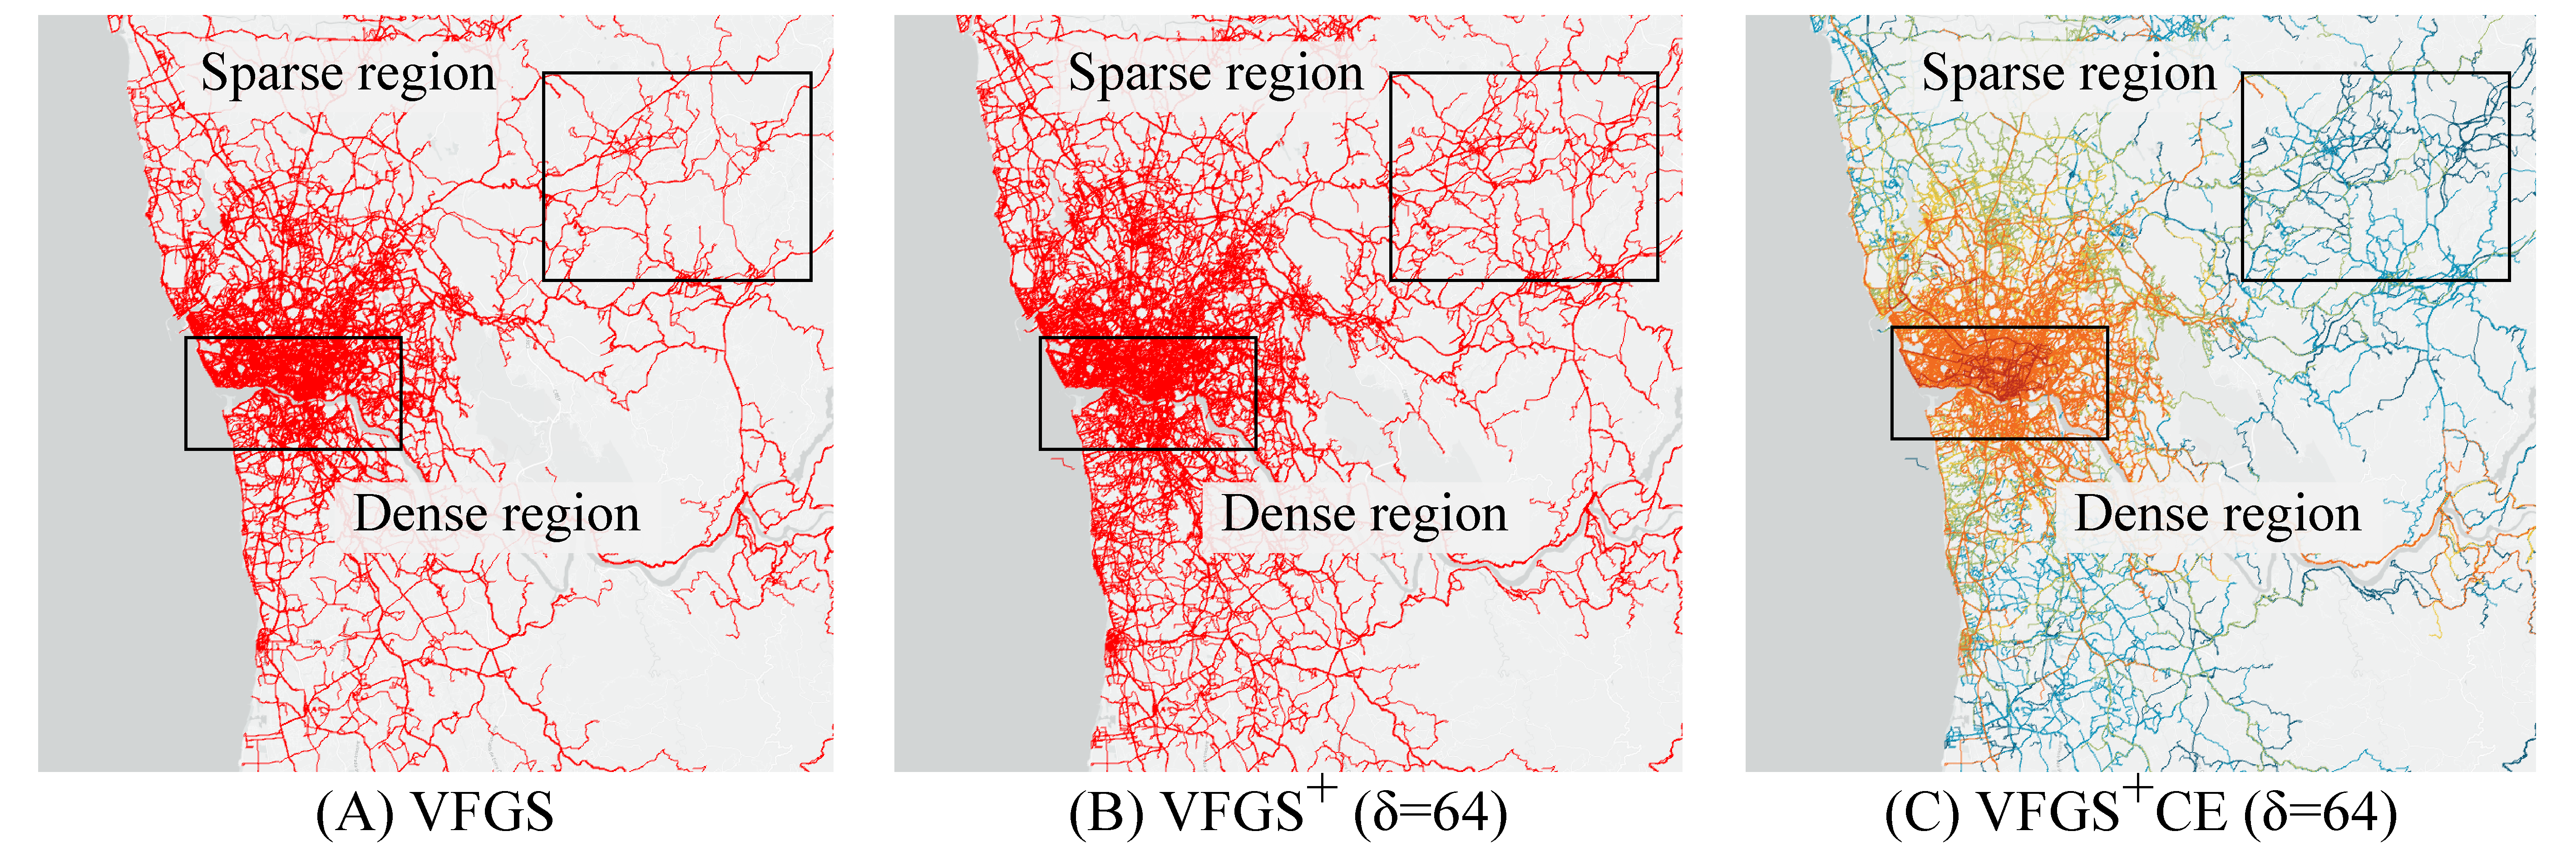
\includegraphics[width=0.44\textwidth]{pictures/problemsolveing/delta_motivation.pdf}
    \vspace{-2mm}
	\caption{Advance approach $\avats$ with \pt{} ($\alpha = 0.5\%$).} \label{fig:delta}
	 \vspace{-6mm}
\end{figure}

%(see Algorithm~\ref{alg:plus})

Taking the above two observations into consideration, the returning result of visual fidelity guaranteed sampling approach $\vats$ could be further improved by
delivering richer information at sparse regions and reducing visual clutter in dense regions.
In this section, we devise an advance approach $\avats$ (see Algorithm~\ref{alg:plus})  to achieve the above two objectives.
Specifically, we introduce perception tolerance parameter $\delta$ in $\avats$, which models human's perception capability at the highest level of details.
In other words, suppose the pixel $(x,y)$ in canvas is covered by result set $\oR$ at the highest level,
the pixels around $(x,y)$, i.e., from $(x-\delta, y-\delta)$ to $(x+\delta, y+\delta)$, are not necessary to cover as they are in the perception tolerance of human beings.

Fortunately, we can slightly revise $\vats$ in Algorithm~\ref{alg:greedy} to incorporate the perception tolerance parameter $\delta$ in advance approach $\avats$.
%, as shown in Algorithm~\ref{alg:plus}.
It measures the contribution of each trajectory $t_i$ w.r.t the selected trajectory set $\oR$'s augmented set $\oR^{+}$, i.e., the selected trajectories and their tolerance pixels.
%(in Line~\ref{line:deltamax}).
%The augmented set $\oR^{+}$ will be updated by the selected trajectory $tmp$ and its tolerance pixels set (in Line~\ref{line:delta}).

%
\begin{algorithm}
    \caption{$\avats(\D,k=\alpha |\D|,\delta)$} \label{alg:plus}
    \begin{algorithmic}[1]
    \State Initialize result set $\oR \leftarrow \emptyset$
    \State Initialize augmented result set $\oR^{+} \leftarrow \emptyset$
    \While{$|\oR| < k$}
        \State $tmp \leftarrow argmax_{t_i \in \D} \oR^{+} \cup t_i$ \label{line:deltamax}
        \State $\oR \leftarrow \oR \cup \{ tmp \}$
        \State $\oR^{+} \leftarrow \oR^{+} \cup \mathsf{augment}(tmp, \delta)$\label{line:delta}
    \EndWhile
    \For{each $t$ in $\D$} \Comment{Representative encoding} \label{line:s}
        \State $tr \leftarrow argmin_{t_i \in \oR}{\mathsf{augment}(t_i, \delta) - t}$
        \State $tr.\mathsf{cnt}++$ \label{line:e}
    \EndFor
    \State Return $\oR$
    \end{algorithmic}
\end{algorithm}


Interestingly, the visual clutter large trajectory visualization problem can be further reduced
by encoding representative trajectories in $\oR$ (the returning result of the advance approach $\avats$) with colors.
In particular, $\avats$ selects the trajectory which has the largest uncovered pixels by taking human's perception tolerance capability into account at each iteration,
instead of only choosing the trajectory with the largest uncovered pixels in $\vats$ (see Algorithm~\ref{alg:greedy}).
During its selection process, some of trajectories will not be included into the result set $\oR$ even they have more uncovered pixels w.r.t. $\oR$.
The reason is their uncovered pixels are too close to the pixels in the selected trajectories, i.e., within the tolerance area of selected pixels.
Taken Figure~\ref{fig:zoom}(A) as an example, suppose $\delta=1$ and trajectory $a$ was selected at the first iteration,
the selected trajectory in the second iteration is $c$ instead of $b$ as almost all pixels in $b$ is in the tolerance area of $a$'s.

Inherently, the $\avats$ trajectory selection process embeds the representativeness of each trajectory in the result set $\oR$.
We define the representativeness of a trajectory as the number of influenced trajectories in the dataset $\D$.
We compute the representativeness of each trajectory in $\oR$, and visualize them by encoding with different colors. %from Line~\ref{line:s} to Line~\ref{line:e} in Algorithm~\ref{alg:plus}
Figure~\ref{fig:delta}(C) shows the visualized result of the  advance approach $\avats$ by encoding the trajectory representativeness with colors.
Obviously, the trajectories in dense region have {darker} color than these in sparse regions as there many trajectories in dense region, thus the selected trajectories in the dense region are more representative.

\begin{figure}[t]
	\centering
	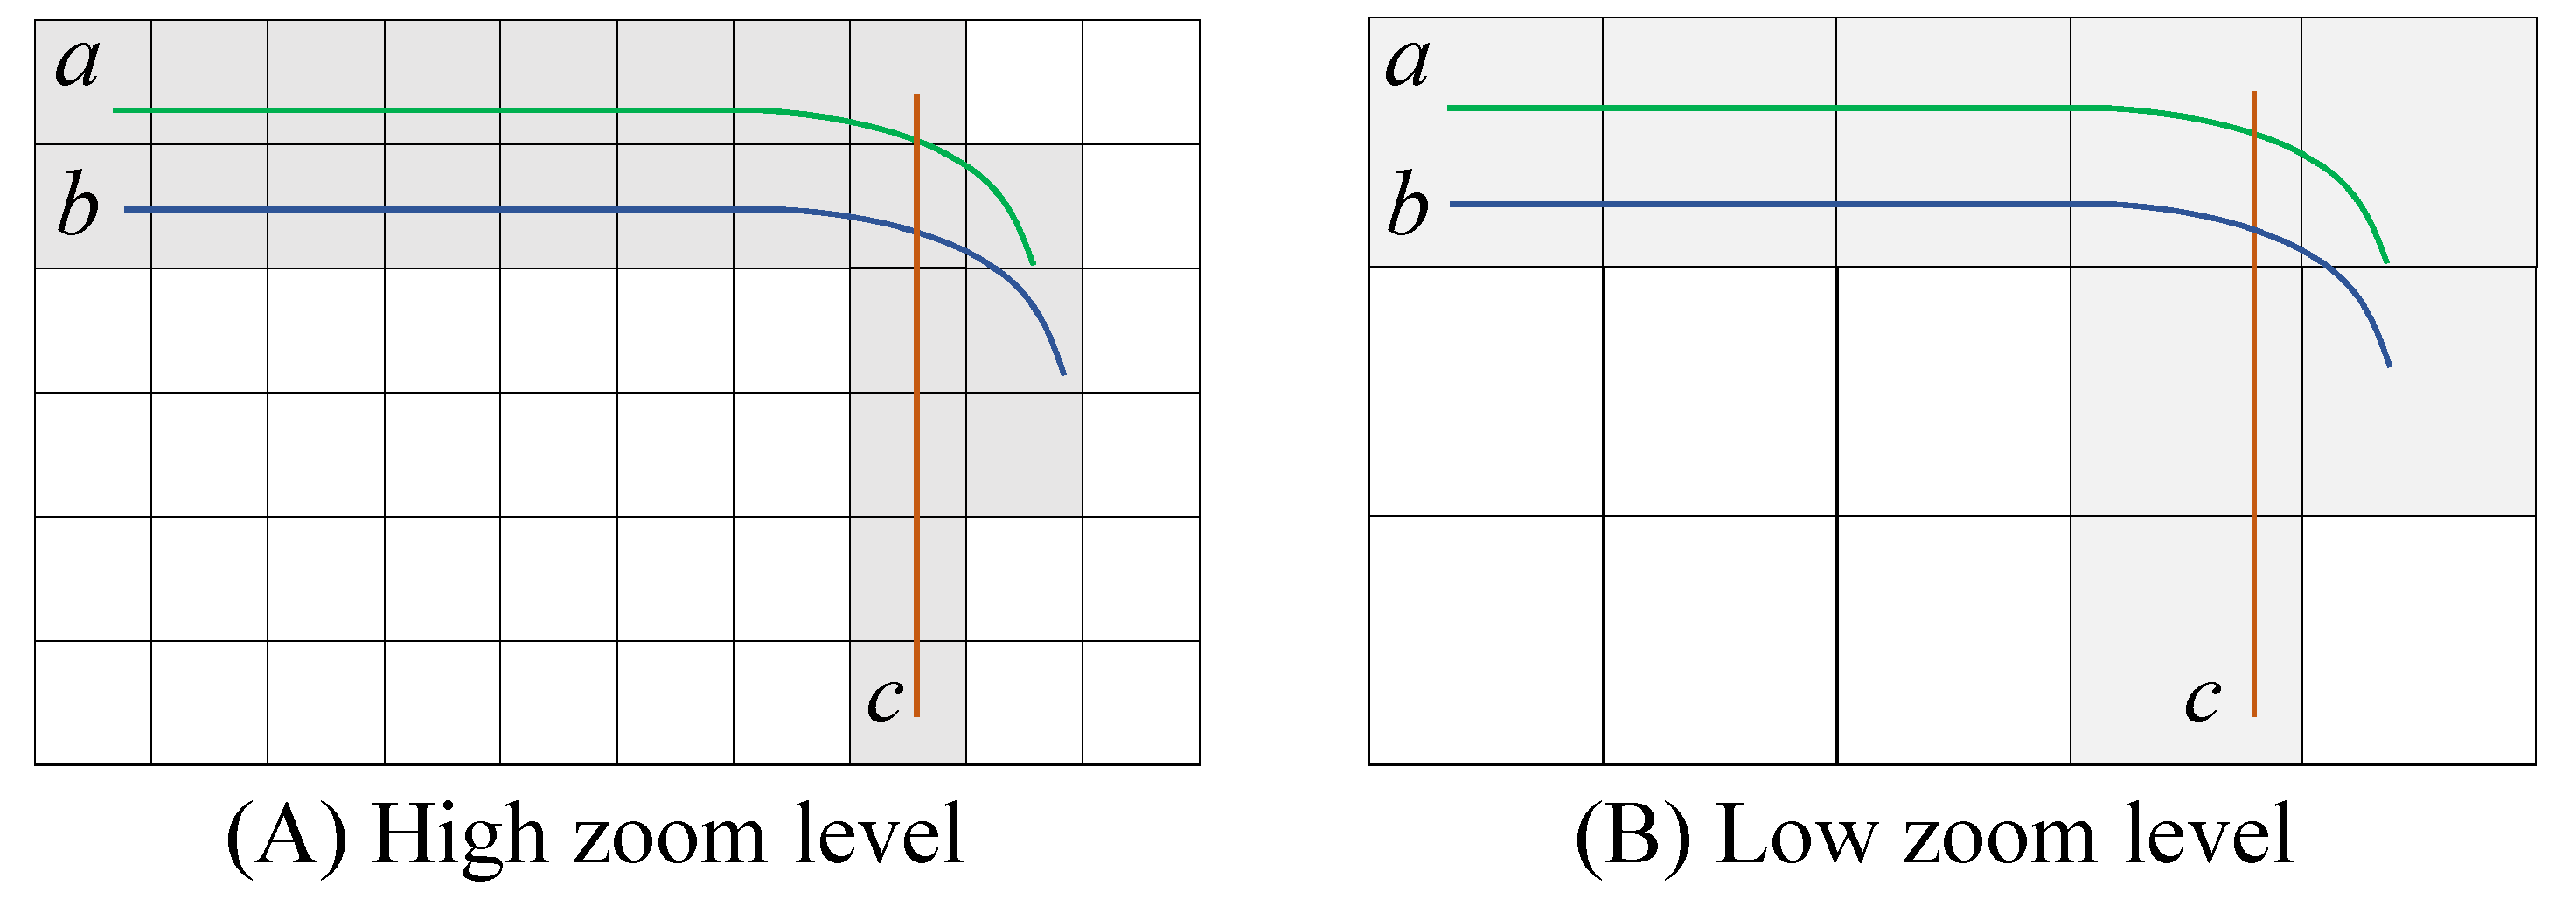
\includegraphics[width=0.4\textwidth]{pictures/problemsolveing/one_to_many.pdf}
	\vspace{-3mm}
	\caption{$\avats$ with different zoom levels.}	\label{fig:zoom} %An illustration of 
    \vspace{-6mm}
\end{figure}


Last but not least, it is worth to point out that our advance approach $\avats$ provides excellent visual fidelity over $\vats$ at arbitrary zooming resolutions naturally.
The key technique to achieve that is it considers the zooming resolutions inherently when introducing the perception tolerance $\delta$.
Take Figure~\ref{fig:zoom} as an example, %Figure~\ref{fig:zoom}(A) and (B) show two different zoom-levels.
the zoom level in Figure~\ref{fig:zoom}(A) is higher than it in Figure~\ref{fig:zoom}(B).
As our above elaboration, our advance approach $\avats$ selects trajectory $a$ and $c$ at Figure~\ref{fig:zoom}(A).
When it zoomed out, as shown in Figure~\ref{fig:zoom}(b), it still captures the main sketch of the underlying dataset (as gray cells shown).




%(1) Richer Information Delivering: details aware; so Arbitrary zooming resolutions
%(2) Popularity Embedding: visual clutter



%\subsection{One-to-many strategy}~\label{sec:one_to_many}
%Since we detect the covered pixels in the highest level, two trajectories may be very close to each other but share very few pixels, which will lead to more information loss in the low zoom view as figure~\ref{fig:one_to_many}.
%We next elaborate a ``one-to-many'' strategy to further optimize the visual quality of our proposed technique.
%Recalling we use the highest zoom level to define the pixel size in the canvas.
%Thus, our visual quality guaranteed sampling algorithm is zoom-level oblivious, e.g., it guarantees the visual quality of result set $\oR$ at every zoom level.
%However, users always do not use/need the highest zoom level in visualization applications.
%For example, Google map shows city and streets at zoom level 1 and 15, respectively~\footnote{\url{https://developers.google.com/maps/documentation/}}.
%Motivated by the above observation, we devise ``one-to-many'' strategy by introducing a visual tolerance parameter $\delta$ to optimize the visual quality for users.
%Specifically, ,
%the ``one-to-many'' strategy will ignore all the pixels around $(x,y)$ within $\delta$ offset distance, i.e., all pixels from $(x-\delta, y-\delta)$ to $(x+\delta, y+\delta)$ will be skipped.
%We will demonstrate the effectiveness of the visual tolerance $\delta$ in experimental evaluations.
%
%%https://developers.google.com/maps/documentation/maps-static/dev-guide#Zoomlevels
%\begin{figure}[t]
%	\centering
%	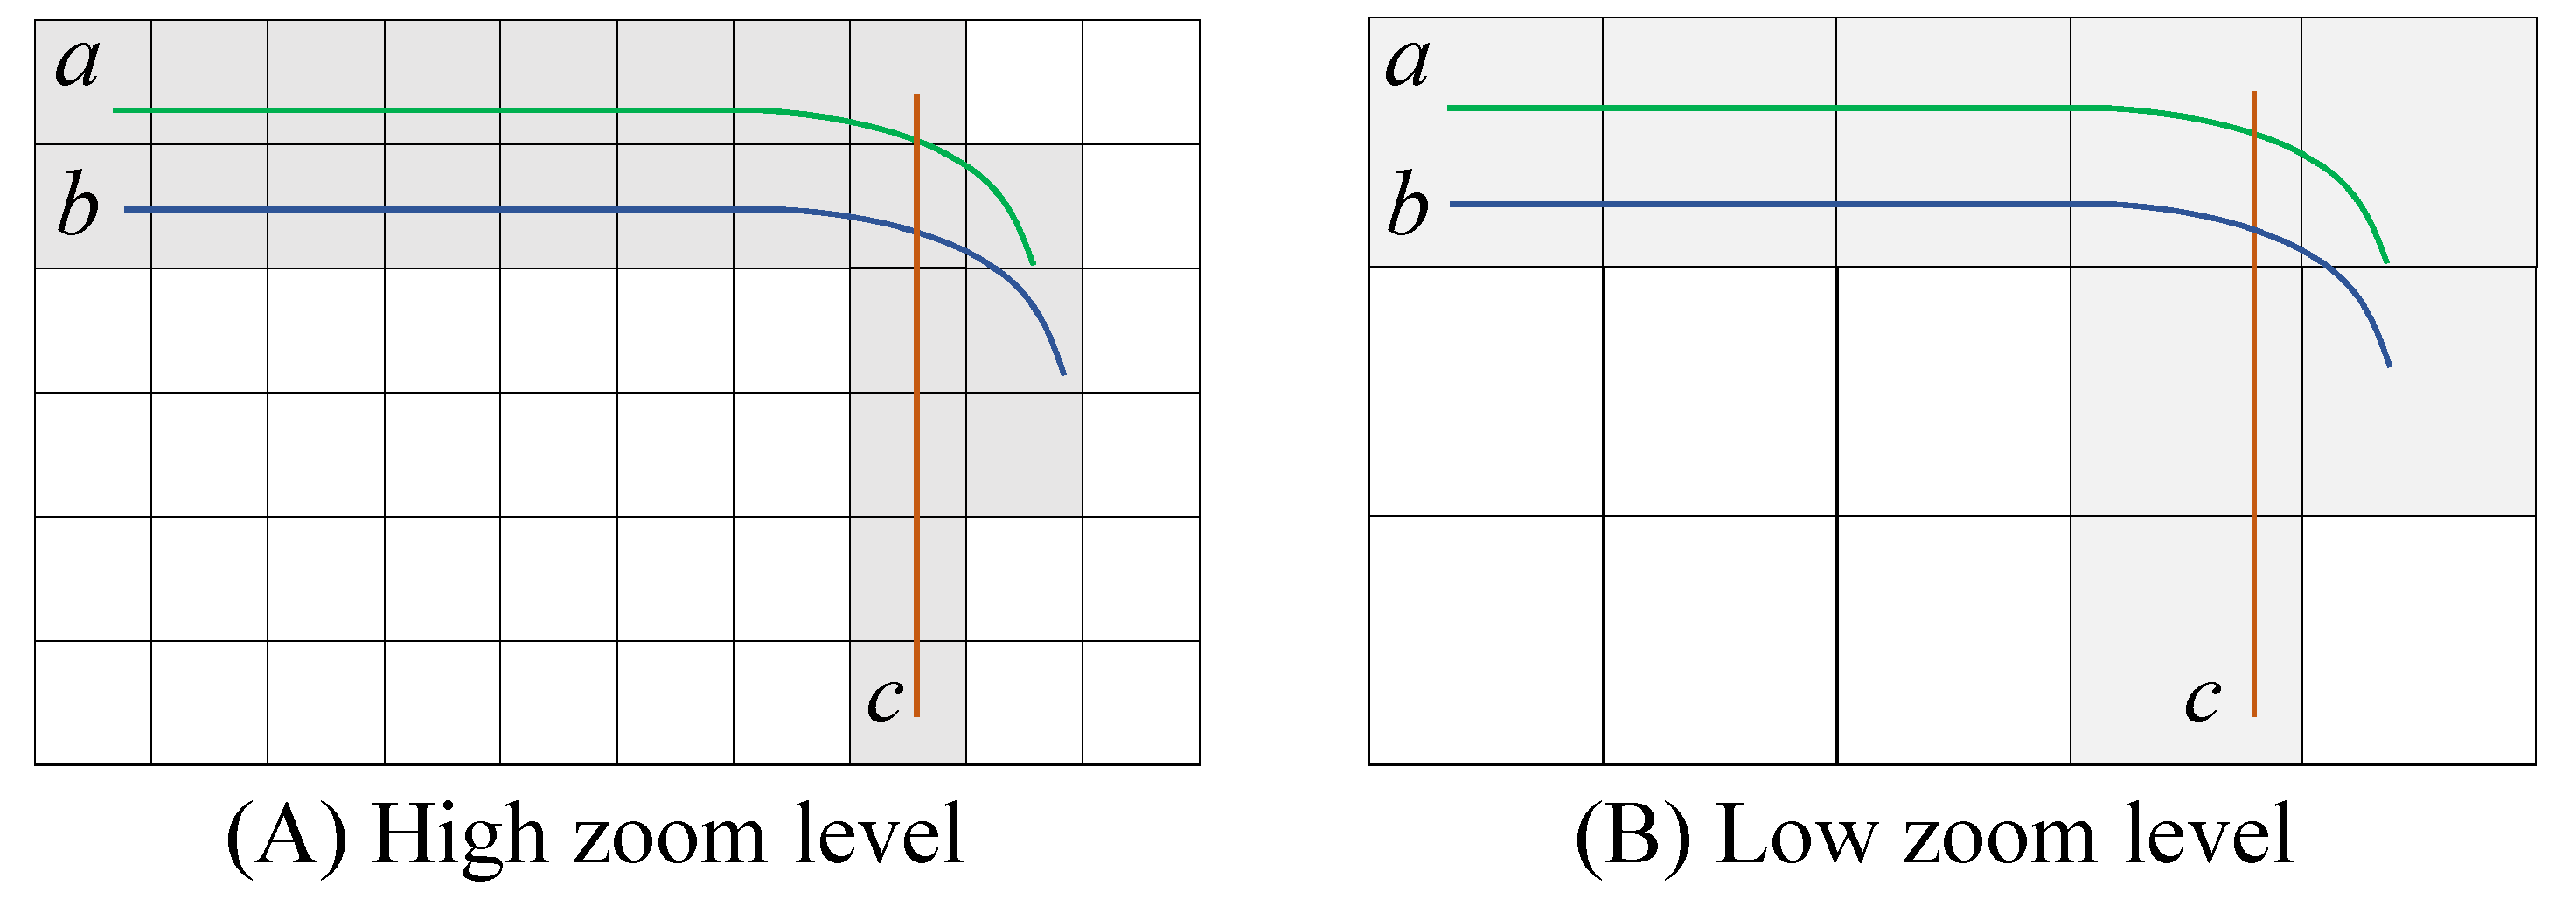
\includegraphics[width=0.4\textwidth]{pictures/problemsolveing/one_to_many.pdf}
%	\vspace{-5mm}
%	\caption{Resolution inconsistency}
%	\vspace{-5mm}
%	\label{fig:one_to_many}
%\end{figure}


%Specifically, $\avats$ incorporates a parameter $\delta$ during trajectory selection process in $\vats$ .
%In particular, we employ the parameter $\delta$ to model the end user's perception ability at the most high level of details.
%Surprisingly, our advance approach $\avats$ not only provides better visualization result when comparing with $\vats$ with the same sampling rate
%(e.g., Figure~\ref{fig:delta}(a) and (b) are the returning result of $\vats$ and $\avats$ respectively),
%but also embeds the popularity of selected trajectories by encoding the rest trajectories in the dataset in them,
%e.g., Figure~\ref{fig:delta}(c) is the visual result of $\avats$ with color encoded popularity.




\section{Experimental Evaluation}\label{sec:exp}
We evaluate our techniques on two real-world datasets, i.e., \pt{} and \sz{}. The trajectory dataset of \pt{}~\cite{pt} has 2.39 million of taxi trajectories, 75.67 million of GPS points in total, its maximum trajectory length is 3,490 GPS points. \sz{}~\cite{sz} includes 3.07 million of taxi trajectories with 53.53 GPS points, the maximum trajectory in it has 2,268 GPS points.
For the sake of page limitation, we briefly present the case of \pt{} in section~\ref{sec:case}, and refer the interested reader to our technical report \cite{techreport} for more cases of \pt{} and \sz{}.

% The trajectories in \pt{} cover several cities around the Porto. 
We then conduct a user study to demonstrate the superiority of our proposal in three real world applications in Section~\ref{sec:user}.
Last, we perform a qualitative evaluation in Section~\ref{sec:quality}.
All experiments are conducted on a machine with Intel i7-8700, 3.2 GHertz CPU, 24 GBytes memory and NVIDIA GeForce GTX1080, 8 GHertz VRAM GPU, running on Windows 10.
We implemented all methods in Java 1.8. The methods call on the Processing 3~\cite{p3} for rendering.
% and has been cleaned for further analysis.

% In Section~\ref{sec:case}, we evaluate the effectiveness of our proposal by the case studies on \pt{} and \sz{} trajectory dataset, respectively.
% We then conduct a user study to demonstrate the superiority of our proposal in three real world applications in Section~\ref{sec:user}.
% Last, we perform a qualitative evaluation in Section~\ref{sec:quality} at last.
% We conducted all experiments on a machine with Intel i7-8700, 3.2 GHertz CPU, 24 GBytes memory and NVIDIA GeForce GTX1080, 8 GHertz VRAM GPU, running on Windows 10.
% We implemented all methods in Java 1.8. The methods call on the Processing 3~\cite{p3} for rendering.


\subsection{Case Study on Porto}\label{sec:case}
% We demonstrate the effectiveness of our proposal by the case studies in \pt{} in Section~\ref{sec:pt} and \sz{} {in Section~\ref{sec:sz}}.

% \subsubsection{Case Studies on \pt{}}\label{sec:pt}
%For the sake of page limitation, we omit the detail elaboration of the cases in Figure~\ref{fig:teaser} and refer the interested reader to our technical report~\cite{techreport}.
%In this section, we present the effectiveness of our proposals with different detail views by investigating three regions of interest in \pt{}, as R1, R2, and R3 shown in Figure~\ref{fig:porto}(A).

We elaborate the cases in Figure~\ref{fig:teaser} to illustrate the effectiveness of our proposal from the following three aspects.


\stitle{Effect of approaches with different zoom-levels}
Considering zoom level 11, Figure~\ref{fig:teaser}(A) is the visualization result of full \pt{} trajectory dataset.
Given the sampling rate $\alpha = 1\%$, Figure~\ref{fig:teaser}(C) and (E) visualized the returning results of uniform random sampling algorithm ($\rand$)
and our advanced visual fidelity guaranteed sampling approach ($\avats$, see Algorithm~\ref{alg:plus}), respectively.
Obviously, Figure~\ref{fig:teaser}(E) looks much more closer to Figure~\ref{fig:teaser}(A) when comparing with Figure~\ref{fig:teaser}(C).
In particular, our proposed $\avats$ not only preserves the visual structure of the full dataset,
but also shows the details of these cities which are far away from the center, as the dashed cycles shown in Figure~\ref{fig:teaser}(E).
However, the details of these dashed cycles in Figure~\ref{fig:teaser}(C), i.e., the returning result from $\rand{}$, are lost.
This issue turns more serious when we zoom in to the details of the visualization results.
Figure~\ref{fig:teaser}(H) and (I) are the visualization result of $\rand$ and $\avats$  (with color encoding) at zoom level 15 with sampling rate $\alpha=1\%$.
Comparing with the visualization result of full dataset at such level, as shown in Figure~\ref{fig:teaser}(G),
the $\rand{}$ in Figure~\ref{fig:teaser}(H) only returns few trajectories and many information in raw data are lost.
Surprisingly, our $\avats$ in Figure~\ref{fig:teaser}(I) captures the main sketch of the full dataset, even with more clear details with the help of color encoding.

\stitle{Effect of sampling rate}
We then evaluate the effect of sampling rate in different approaches.
Figure~\ref{fig:teaser}(B) and (C) are the visualization results of $\rand{}$ with sampling rate $0.1\%$ and $1\%$, respectively.
Figure~\ref{fig:teaser}(D) and (E) visualized the returning trajectory sets of our $\avats{}$ with sampling rate $0.1\%$ and $1\%$, respectively.
We then have the following observations:
(i) the larger sampling rate, the better visual fidelity of the visualization results, e.g.,
Figure~\ref{fig:teaser}(C) and (E) are more closer to Figure~\ref{fig:teaser}(A) when comparing with Figure~\ref{fig:teaser}(B) and (D), respectively;
(ii) the visualization result of $\avats$ with sampling rate $0.1\%$ in Figure~\ref{fig:teaser}(D)
performs even more better than the result of $\rand{}$ with sampling rate $1\%$ in Figure~\ref{fig:teaser}(C) to capture the visual structure of the full dataset in Figure~\ref{fig:teaser}(A).


\stitle{Effect of color encoding}
% Next, we present the superiority of color encoding scheme in $\avats$, which denotes as $\cavats$ in subsequent sections.
\QM{Given zoom level 11 and sampling rate $1\%$, Figure~\ref{fig:teaser}(E) and (F) are the visualization results of our $\avats$ and $\cavats$ (i.e., $\avats$ with color encoding), respectively.
It is worth to point out the visual clutter in the visualization result generated by full dataset and $\avats$ are serious, as shown in the embedded rectangles of  Figure~\ref{fig:teaser}(A, E).
However, the visualized result of $\cavats$ in Figure~\ref{fig:teaser}(F) reduces the visual clutter by encoding the trajectory distribution by color, which provides a clear visual structure of the input dataset. 
In addition, the comparison of the visualized results in Figure~\ref{fig:teaser}(G) and (I) confirms the effectiveness of our proposed color encoding scheme for visual clutter in large dataset again.}
%\begin{figure*}
%	\centering
%	\includegraphics[width=0.85\textwidth]{pictures/experiment_study/case_porto.pdf}
%	\vspace{-3mm}
%	\caption{Effectiveness studies of $\avats$ at dense and sparse regions with detail visualizations in \pt{}.}
%	\label{fig:porto}
%    \vspace{-3mm}
%\end{figure*}
%
%\stitle{Sparse region R1}
%R1 is a sparse region and has few trajectories, as the visualization result of full \pt{} dataset shown in Figure~\ref{fig:porto}(B1).
%The reason is the two cities Paredes and Penafiel in R1 are far away from the center of Porto.
%Given sampling rate $\alpha=0.5\%$, Figure~\ref{fig:porto}(B2), (B3) and (B4) are the visualization results of the returning trajectory set from $\rand{}$, $\vats$ and $\avats$ with $\delta=64$, respectively.
%As our above statement, the result of $\rand$ almost misses all information in sparse region.
%While $\vats$ performs much better than $\rand$ as it provides theoretical visual fidelity guarantee, but it still lost detail information.
%Taking Figure~\ref{fig:porto}(B1) as reference, the trajectory bundle and trajectory structure are lost in Figure~\ref{fig:porto}(B3$a$) and (B3$b$).
%As expected, our advanced approach $\avats$ in Figure~\ref{fig:porto}(B4) with perception tolerance value $\delta=64$ did an excellent job to capture the details in the full dataset when comparing with $\vats$ in Figure~\ref{fig:porto}(B3).
%As shown in Figure~\ref{fig:porto}(B4$b$), the trajectory sketch of Penafiel is almost the same as it in Figure~\ref{fig:porto}(B1$b$), the visualized result of full dataset.
%
%\stitle{Median region R2} It is near to the center of Porto, which has more taxi trajectories than R1, see Figure~\ref{fig:porto}(A).
%As noted in Figure~\ref{fig:porto}(C1), R2 includes three cities: Ermesinde, Rio Tinto and Valongo.
%Figure~\ref{fig:porto}(C2) and (C3) visualized the returning result of $\avats$ with perception tolerance value $\delta=4$ and $64$, respectively.
%Visually, Figure~\ref{fig:porto}(C3) has more trajectory branch details than Figure~\ref{fig:porto}(C2), as the rectangles $c$ and $d$ shown in them.
%Figure~\ref{fig:porto}(C4) is the result of $\cavats$, i.e., it colors the trajectories by their representativeness.
%Intuitively, Figure~\ref{fig:porto}(C4) shows its superiority over Figure~\ref{fig:porto}(C3) to capture the trajectory distributions.
%For example, the color of the region $f$ in Figure~\ref{fig:porto}(C4) is {darker} than the rest two regions $e$ and $g$.
%Thus, we can conclude Rio Tinto (region $f$) has more taxi trajectories than other two cities, which is hard to be concluded via Figure~\ref{fig:porto}(C3), even Figure~\ref{fig:porto}(C1), the visualization result of full dataset.
%It verified that the color encoding scheme could enrich the visual information in large trajectory visualization.
%
%\stitle{Dense region R3} It is the center of Porto, which has the highest concentration of the trajectories and causes serious visual clutter, as visualized in Figure~\ref{fig:porto}(D1).
%For example, the structure of trajectories in Figure~\ref{fig:porto}(D1$i$) is unclear.
%$\avats$ with $\delta=4$ alleviates the visual clutter and preserves the trajectory distribution, see Figure~\ref{fig:porto}(D2).
%Figure~\ref{fig:porto}(D3) visualized the result of $\avats$ with $\delta=64$, which enhances the visual fidelity of Figure~\ref{fig:porto}(D2).
%Specifically, it preserves more details (see rectangle $h$) and has a more clear structure in the {densest} region (see rectangle $i$).
%Visually, Figure~\ref{fig:porto}(D4) is the best among these four visualization results.
%It confirms the advantages of color encoding scheme in $\cavats$.

% \subsubsection{Case Studies on \sz}\label{sec:sz}
% We further evaluate the effectiveness of our approaches by using the taxi trajectories in Shenzhen, China.
% The \sz{} trajectory dataset has many different characteristics with \pt{}, e.g., trajectory distribution, city centers, and taxi move patterns.
% We set sampling rate $\alpha=1\%$ and perception tolerance value $\delta = 64$ in this section.

% \begin{figure*}[t]
% 	\centering
% 	\includegraphics[width=0.85\textwidth]{pictures/experiment_study/case_shenzhen.pdf}
% 	\vspace{-4mm}
% 	\caption{Case studies on \sz{} taxi trajectory dataset, sampling rate $\alpha = 1\%$.}
% 	\label{fig:shenzhen}
%     \vspace{-3mm}
% \end{figure*}

% \stitle{Overview of Shenzhen}
% Figure~\ref{fig:shenzhen}(A) is the visualization result of full \sz{} dataset at zoom level 11.
% The dense regions in southern of Shenzhen, as the dashed circles shown in Figure~\ref{fig:shenzhen}(A), are \emph{Baoan, Nanshan, Futian} and \emph{Luohu} districts,
% which are the most prosperous commercial regions in this city.
% The returning results of $\rand$, $\avats$ and $\cavats$ are visualized in Figure~\ref{fig:shenzhen}(B), (C) and (D), respectively.
% Not surprisingly,  the visualized result of $\rand$ in Figure~\ref{fig:shenzhen}(B) is quite different from the full dataset in Figure~\ref{fig:shenzhen}(A).
% $\avats$ in Figure~\ref{fig:shenzhen}(C) shows it superiority by capturing the overview of \sz{} dataset and even preserves the isolated trajectories,
% as highlighted in left-upper corner of Figure~\ref{fig:shenzhen}(C).
% It owes to $\avats$ provides theoretical visual fidelity guarantees on the returning result set.
% $\avats$ with color encoding $\cavats$ further improved the visual fidelity of $\avats$.
% Specifically, both Figure~\ref{fig:shenzhen}(A) and (C) are suffering from visual clutter seriously,
% e.g., it is unable to recognize the main roads in the circles $a$ and $b$ as both are full with trajectories.
% However, the result of $\avats$ with color encoding, as shown in Figure~\ref{fig:shenzhen}(D), reduce the visual clutter perfectly.
% For example, it is clear that the main roads of circle a and b are these roads with {darker} colors in Figure~\ref{fig:shenzhen}(D).

% We then present the advantages of our $\avats$ in two representative areas, i.e., airport and North railway station, in \sz{} dataset.

% \stitle{Airport in Shenzhen}
% Comparing with visualization result of full dataset in Figure~\ref{fig:shenzhen}(E),
% the visualized result of $\rand$ in Figure~\ref{fig:shenzhen}(F) only includes very few trajectories.
% both $\avats$ and $\cavats$ (see Figure~\ref{fig:shenzhen}(G) and (H)) reserve the major structure of the airport area excellent.
% Moreover, $\cavats$ provides richer information by computing the representativeness of trajectories.
% For example, the taxi trajectories which pass through G4 and G104 is more than that in Baoan Avenue.
% The reason is that the colors of G4 and G104 is {darker} than Baoan Avenue, as highlighted in Figure~\ref{fig:shenzhen}(H).

% \stitle{North railway station in Shenzhen}
% We next investigate the visualizations of the full dataset, uniform random sampling result set, and visual fidelity guaranteed sampling result set around North railway station of Shenzhen, which are shown from Figure~\ref{fig:shenzhen}(I) to (L).
% Interestingly, $\avats$ and $\cavats$ visualized the overpass near North railway state clearly, as circle $c$ shown in both Figure~\ref{fig:shenzhen}(K) and (L).
% Due to visual clutter, the overpass is not clear in Figure~\ref{fig:shenzhen}(I), which visualized the full dataset.
% It even disappeared in the visualized result of $\rand$ in Figure~\ref{fig:shenzhen}(G).
% Moreover, it is easy to compare the traffic flows in different roads via $\cavats$ visualization result.
% For example, the road G94 has a higher road traffic flow than the Minzhi Avenue and Meilong Avenue, as different colors shown in Figure~\ref{fig:shenzhen}(L).

\subsection{User Study}\label{sec:user}
In this section, we conduct an extensive user study on three real-world applications, i.e., region center identification, reachable route inspection, and traffic flow comparison, to demonstrate the superiority of our proposal.
% We present our user study setting in Section~\ref{sec:uset}, and analyze the user study results in Section~\ref{sec:uret}.

%To further evaluate the effectiveness of $\avats$ from the the audience perspective, we conducted formal user studies to compare how users perform the urban exploration tasks with visualizations generated by whole dataset, random sampling and $\avats$.


\begin{figure}[t]
	\centering
	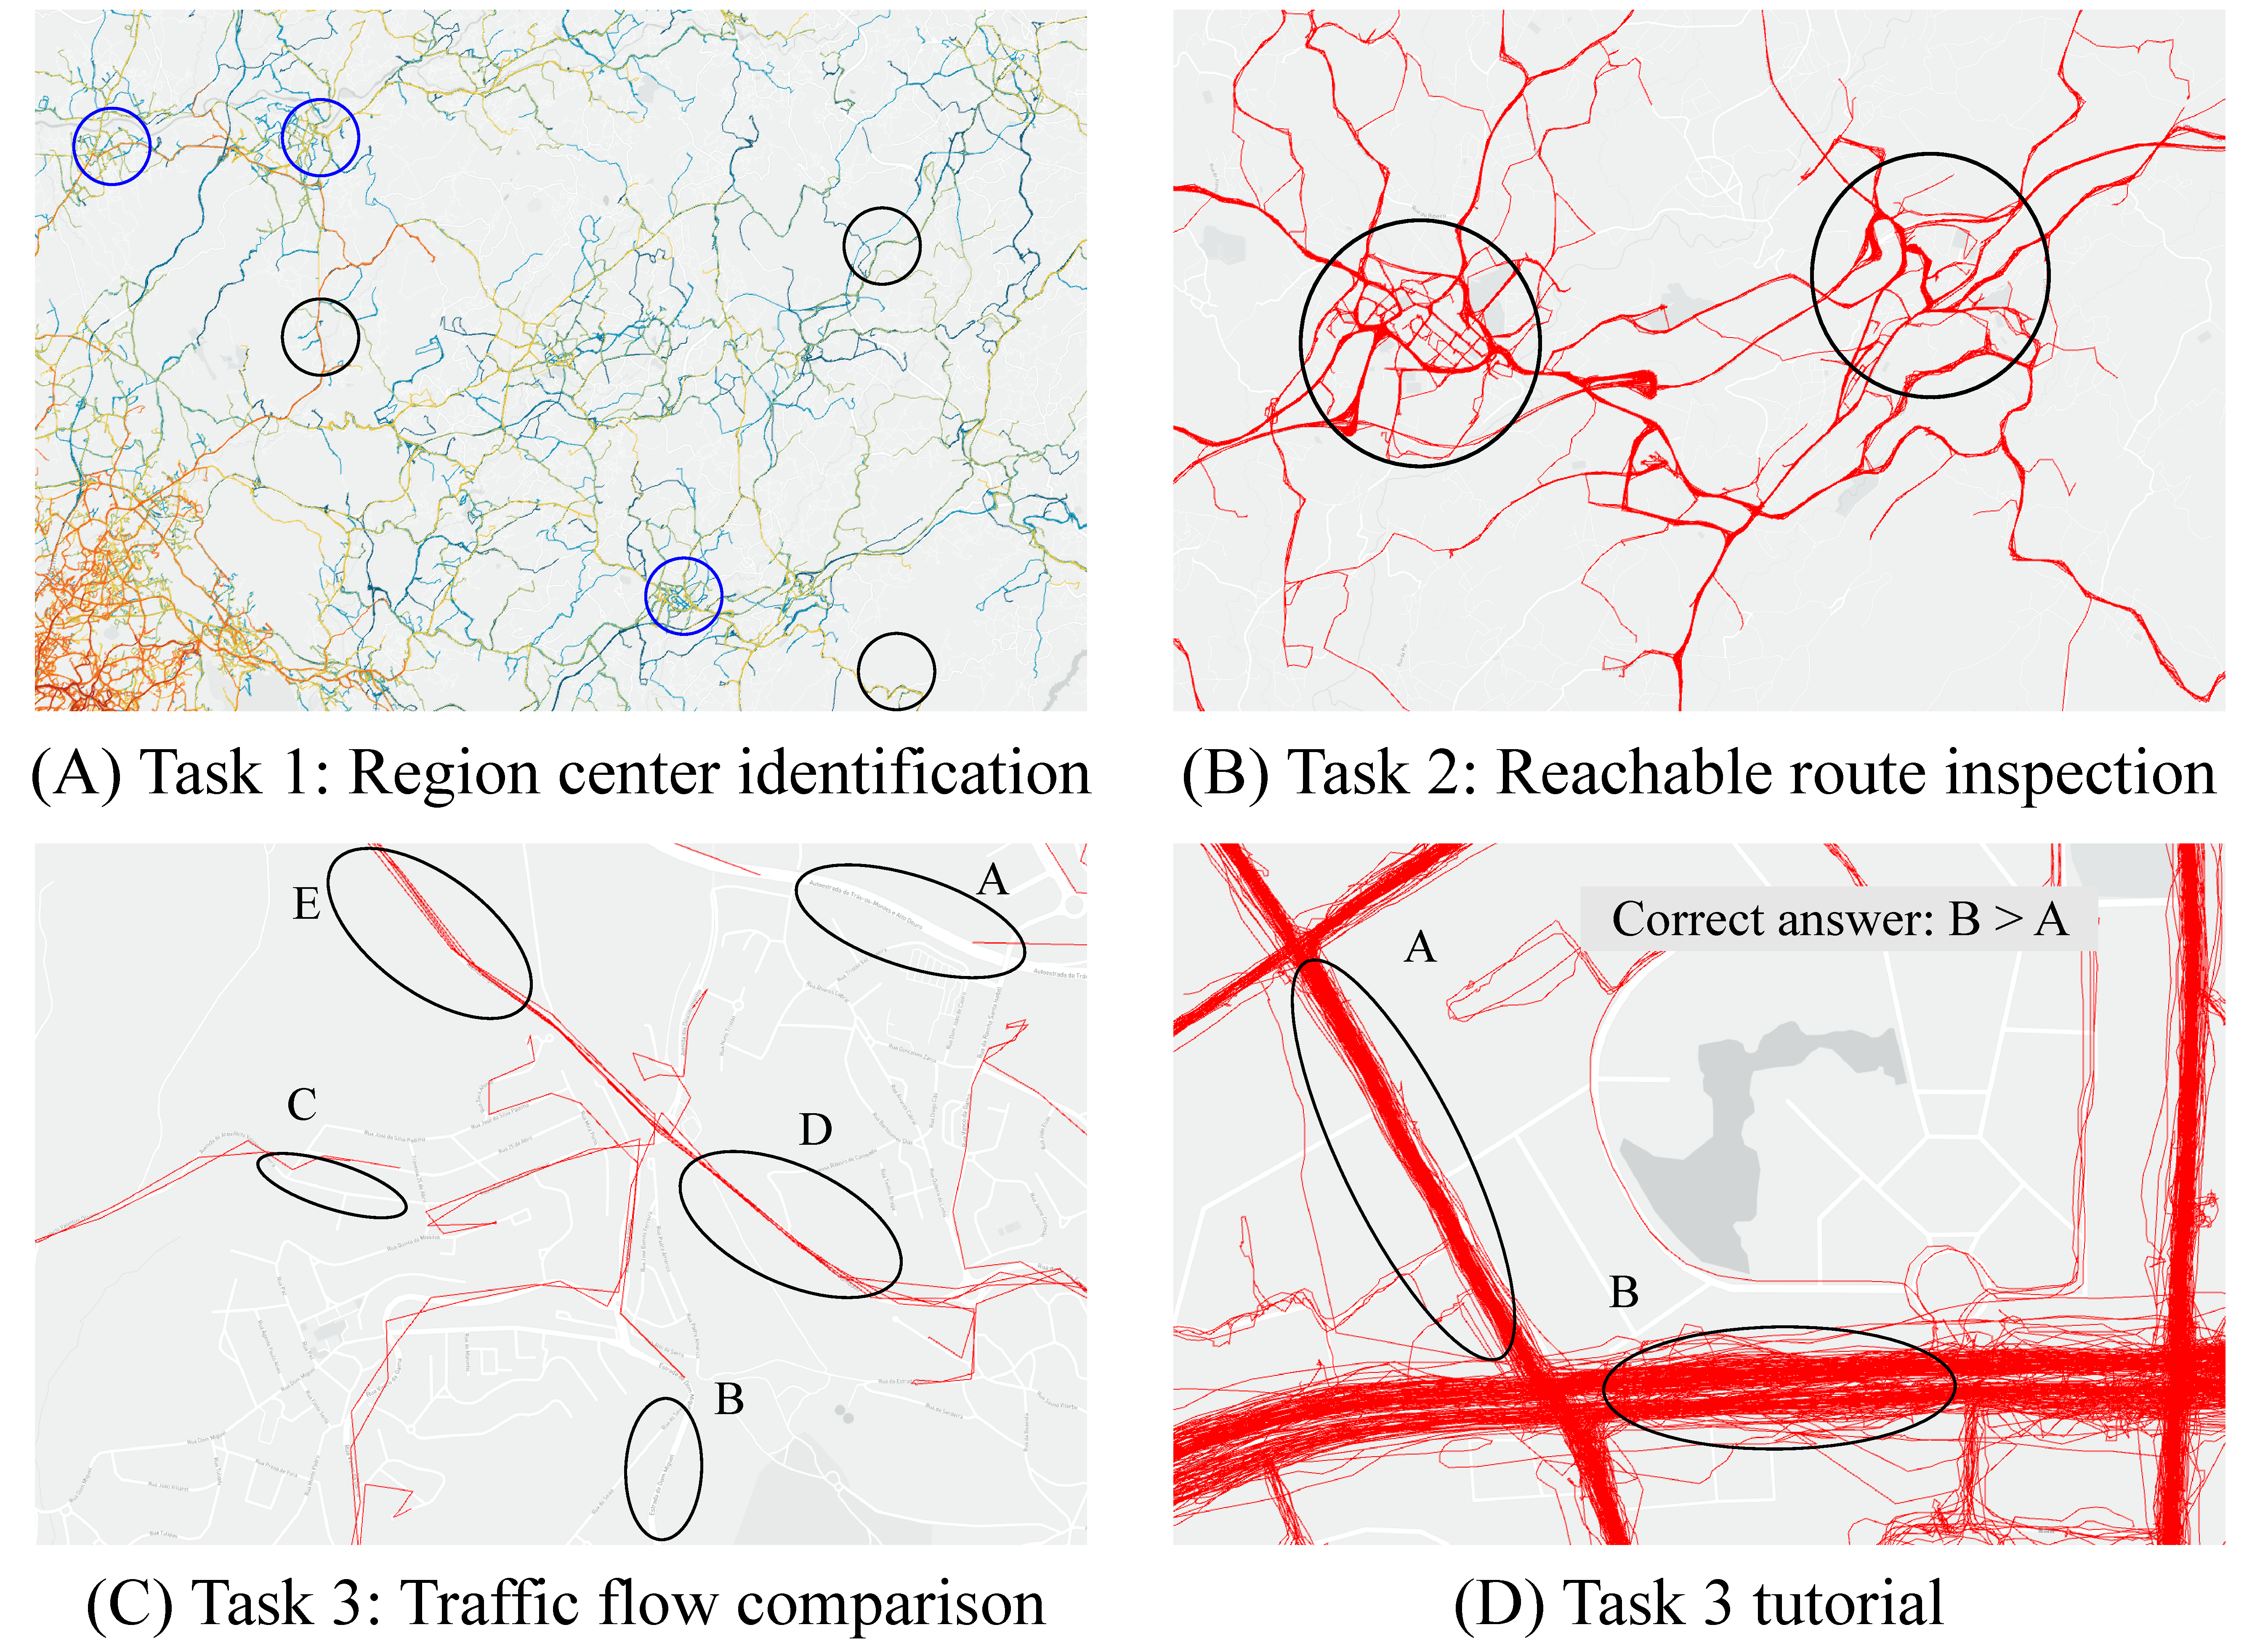
\includegraphics[width=0.40\textwidth]{pictures/user_study/interface.pdf}
	\vspace{-3mm}
	\caption{Three tasks in user study.}
	\label{fig:apps}
	\vspace{-6mm}
\end{figure}

\subsubsection{User study setting}\label{sec:uset}

\stitle{Participants and apparatus}
We recruited 186 participants (24 females, 162 males, aged 18 to 29 with mean=21.16, standard derivation =1.48) .
% with normal vision or normal corrected vision.
% All participants have the background of computer science.
%, 4.84\% of them have data visualization background.
%The user study system is a web-based platform, which has the size-fixed interface and the participants perform the user study on their own  computers.
%Considering the unfairness caused by different screen sizes, we recommend all participants to set the screen resolution as 1980*1080.
%All images displayed on the interface have the same size 450*300.
The user study system is a web-based platform, all displayed visualization views are with size 450*300.
% All participants performed the user study on their own computers.


\stitle{Studied visualization results}
We use the taxi trajectory dataset of \pt{} and \sz{} for the user study.
% We study the visualization results generated by different approaches in three real-world tasks.
% We first introduce the studied data generation methods then elaborate the tasks shortly.
The visualization results we investigated in user study are: (i) full dataset $\full$,
(ii) the result sets of $\rand$,
(iii) the result sets of $\vats$  (see Algorithm~\ref{alg:greedy}),
(iv) the result sets of $\avats$ ,
and (iv) the result sets of $\avats$ with color encoding (see Algorithm~\ref{alg:plus}), i.e., $\cavats$.
The sampling rate is $\alpha = 0.5\%$ and perception tolerance value $\delta = 64$ in all the visualization results in the user study section.
% In each task, we use the identical regions with different visualized trajectories, which are returned from the above approaches.


\stitle{User study tasks}
\QM{All participants were asked to performed three tasks:}  
% (T1) region center identification, (T2) reachable route inspection, and (T3) traffic flow comparison.
%as shown in Figure~\ref{fig:apps}(A), (B), and (C), respectively.

\sstitle{(T1) region center identification}
\QM{The center of the city or commercial region plays an important role in traffic management.
Consequently, the passing taxi trajectories of these centers are more than its surrounding ares, and result in a star-shape cluster of trajectories in the visualization.
% In this task, we randomly selected 6 different regions which include city or commercial centers from \pt{} and \sz{}.
% For each region, we asked the participants to identify the correct city/region center(s) in it.
T1 had 30 visualizations which include city or commercial centers from \pt{}.
% For each visualization views,  we labelled the locations of the {city or commercial region} centers in it as the correct centers at first.	
% We then randomly selected other {locations} far away from the correct centers, and labelled them as incorrect ones.
% We fixed the number of correct centers in each visualization view as 3.
For each visualization,  we manually labelled 3 locations of the city or commercial region centers in it as the correct centers.	
We then randomly generate three locations far away from the correct centers, and labelled them as incorrect ones.
Each participant will perform T1 on 6 different visualizations selected randomly.
As shown in Figure~\ref{fig:apps}(A), the participants needed to identify 3 correct centers among these 6 cycles by clicking the corresponding cycles.}

\sstitle{(T2) reachable route inspection}
Intuitively, the visualized trajectories indicate the reachable routes which connect different regions.
In this task, we gave a visualization view with two circular areas, as illustrated in Figure~\ref{fig:apps}(B),
then asked the participates to inspect the representative reachable routes between these two areas.
We assumed the more trajectories in that route, the more representative it is.
For each visualization view, the number of reachable routes was given.
In T2, we randomly selected 7 different regions, each of them includes two or more cities/commercial districts.
For the 5 different visualization views of a selected region, we chose two identical circular areas in each of them randomly.
%, which visualized the returned trajectory set of different approaches.


\sstitle{(T3) traffic flow comparison}
In practical, a road with large traffic flow has lots of passing trajectories, thus it results in a denser and broader trajectory brunch in the visualization.
In the trajectory visualization with color encoding, such kind of pattern can also be highlighted by a concentration of trajectories with {dark} color.
%It is important to preserve the traffic flow information during large trajectory visualization.
In this task, we asked the participates to compare the traffic flows in two roads by the visualization results, as shown in Figure~\ref{fig:apps}(C).
In particular, the participants were asked to choose the road with larger traffic flow by clicking the radio box.
They also could choose ``I am not sure'' if they could not decide the answer.
T3 included 5 randomly selected regions and each of them had a clear road structure.
It had 25 visualization views and 60 road pair comparisons in total.
We counted the number of passing trajectories in each road as the exact traffic flow in it.




%\textbf{T1. City/commercial region center identification.}
%% what participants do
%As shown by Figure~\ref{fig:user_study}(C), a visualization view was given and several regions were marked by circle. The participants needed to select the regions which could be city/commercial centers by click the corresponding circles. In each task, the number of correct regions were given.
%%Why possible
%The city or commercial region centers always have more passing trajectories from different directions than the surrounding regions, which results in the \UC{start-shape} cluster of trajectories in the visualization.
%%Generate the data
%To generate the test data of T1, we randomly chose several visualization views which contain city/commercial regions and labeled the locations of each city/commercial region center on the visualization as the correct locations first.  Then we randomly generated locations and remove the locations close to the correct locations, the remaining locations are the error locations. In each task of T1, with a given visualization, the same number of correct and wrong locations will be randomly selected.
%
%\textbf{T2. Reachable route inspection.}
%% what participants do
%Figure~\ref{fig:user_study}(D) shows the interface of T2, which includes a visualization and two circular regions. The users needed to draw several most representative reachable routes to connect the two regions. The number of the reachable routes is given.
%%Why possible
%The reachable routes indicate the routes connecting two regions, these routes must have the passing trajectories.
%%Generate the data
%To generate the test data, we randomly chose the visualization views which contain two or more city/commercial regions. In each task of T2, a visualization and two regions were randomly selected.

%\textbf{T3. Traffic flow estimation}.
%% what participants do
%As shown by Figure~\ref{fig:user_study}(B), with a given visualization, some road segments will be identified by ellipses(shown as~\ref{fig:user_study}(B)). Several road segment pairs were randomly selected and listed below the view. The participants were asked to choose the one with larger traffic flow by clicking the radio box. They can also choose ``I am not sure'' if they cannot decided the answer.
%%Why possible
%
%%Generate the data
%To generate the test data of T3,  we sampled and selected the visualization views which contain clear road structures. Then the number of trajectories passing through each road segment was counted as the traffic flow.



\stitle{User study procedure}
In the user study system, we first provided a brief introduction about the motivation, tasks and visual encoding scheme, then followed by three tasks.
In each task, we included a tutorial (with the correct result) to help the participants familiarizing themselves with the interface, interaction and tasks.
For example, Figure~\ref{fig:apps}(D) shows a tutorial of T3 in Figure~\ref{fig:apps}(C), where the traffic flow in road A is smaller than it in road B, as the correct answer shown in it.
We then randomly chose different views with different questions in each task for different participates.
After they completed all the questions, their answers were collected and saved in the database for the result analysis.
At last, post-interviews were conducted to collect the feedback of the participants.
We refer the reviewers to our supplementary video for the details of our user study tasks and procedure.
%To evaluate the answers given by the participants, we refer the reviewers to our supplementary video for details of our user study procedure.

%The user study began with the introduction which introduces the motivation, tasks and visual encoding.
%Then the following sessions are divided into three blocks according to the task types. Each block starts with a task tutorial, in which the participants could perform several demo tasks, thus familiarizing themselves with the interface, interaction and tasks. For example, Figure~\ref{fig:user_study}(A) shows the demo task of T3, in which the users can check the correct answer after clicking the ``check'' button. After all the questions are finished, the answers and time usage are collected and saved in the database for the further analysis.

\subsubsection{User study result analysis}\label{sec:uret}
%\TB{Figure~\ref{fig:accuracy} depicts the average accuracy of the different visualization approaches on different tasks from all user study participates.
%Given a task with specified approach, we visualize the average accuracy of all questions by a colored circle and a line-segment to indicate the highest and lowest score of all questions of this task.}
Figure~\ref{fig:accuracy} depicts the average accuracy of all five approaches applied in the three user study tasks.


%\begin{figure}[t]
%	\centering
%	\includegraphics[width=0.40\textwidth]{pictures/user_study/accuracy.png}
%	\vspace{-4mm}
%	\caption{Average accuracy of three types of tasks. X axis indicates the task types. Y axis indicates the accuracy of different approaches.}
%	\label{fig:accuracy}
%	\vspace{-6mm}
%\end{figure}

\begin{figure}[t]
	\centering
	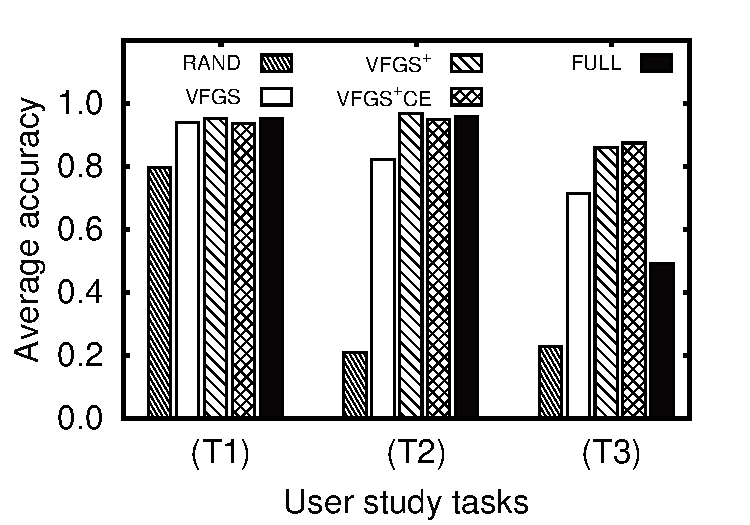
\includegraphics[width=0.3\textwidth]{pictures/userstudy}
	\vspace{-4mm}
	\caption{Average accuracy of three user studied tasks. X axis shows three tasks. Y axis indicates the accuracy of different approaches.}
	\label{fig:accuracy}
	\vspace{-6mm}
\end{figure}

For (T1) region center identification task, the average accuracy of our proposed approaches (i.e., $\vats$, $\avats$, and $\cavats$) are higher than that of $\rand{}$.
Moreover, our proposed approaches have a very close similar performance with visualizing the full dataset $\full$.
It means the visualized returning results of our proposed approaches worked as excellent as the full data visualization for the exploration of human activity center application.
We observed that the performance of $\cavats$ is slightly worse than the performances of $\avats$ and $\full$.
In the post-interviews, some of the participants said that the color of trajectories may distract user's attention and make the cluster characteristics not obvious.


%the participants using all the three proposed methods had a very close performance with the participants using whole dataset, indicating the proposed methods can replace the whole dataset with a guaranteed performance in the exploration of human activity center with trajectory visualization.

For (T2) reachable route inspection task, it is no doubt the $\rand$ has the worst performance among these 5 visualization approaches as it lost many (if not all) detail information.
Unlike \QM{T1, T2} are always performed at a fine-grained level of visualization,
which requires good preservation of the details, especially for the sparse regions with few trajectories.
Thus, the advantages of our advance approaches $\avats$ and $\cavats$ over $\vats$ become obvious and clear.
The reason is that our advance approaches considered the data distribution and perception tolerance explicitly.
%It also is worth to point out our $\avats$ (with average accuracy 0.968) outperforms the visualizations of $\full$ (with average accuracy 0.959) slightly.

%Interestingly,
%For the tasks of T2, $\avats$, $\avats$ with color encoding and the whole dataset all have similar accuracy scores which are far higher than random sampling.
%Moreover, $\avats$ and $\avats$ with color encoding also outperforms the $\vats$ clearly by taking the perception parameters into consideration.
% This results demonstrate the advantage of $\avats$ on the urban exploration at a detail level.


Visually, the task of traffic flow comparison in (T3) is more difficult than (T1) and (T2), which results in relatively lower average accuracy for all approaches.
As expected, $\rand$ is the worst.
Interestingly, the average accuracy of visualization views of $\full$ is lower than our proposed approaches, i.e., $\vats,\avats$ and $\cavats$.
In the post-interviews, the participants pointed out that many visualization views of $\full$ had serious visual clutter,
which made it is impossible to compare the traffic flows in the two road segments.
The average accuracy of our proposed $\avats$ shows $\avats$ alleviated the visual clutter problem and preserved the clear structure.
$\cavats$ further highlighted the crowded road segments from the surroundings by color, which {resulted in} the highest average accuracy in the task (T3).

In summary, the qualitative user study of our proposal demonstrates the effectiveness of $\avats$ for large trajectory visualization by three real-world tasks.
All of our proposals ($\vats$, $\avats$, and $\cavats$) outperform the $\rand$ approach significantly.
In addition, the participates achieved equivalent or higher accuracy scores in $\avats$ and $\cavats$ when comparing with the visualization of $\full$.

%\vspace{-2mm}
\subsection{Qualitative Evaluation}\label{sec:quality}
In this section, we conduct a qualitative evaluation of our proposals on \pt{} and \sz{} trajectory datasets from two aspects: (i) the visual fidelity in different zoom levels,
and (ii) the running time with different sampling rates.

\begin{figure}
 \centering
 \small
 \begin{tabular}{cc}
   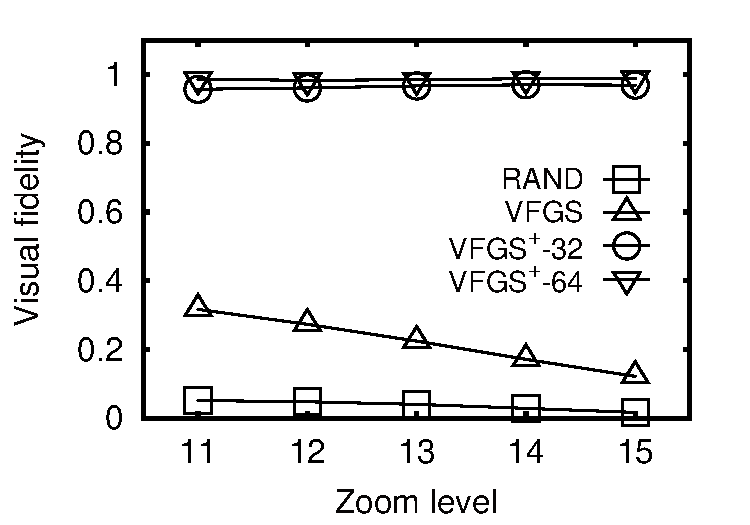
\includegraphics[width=0.44\columnwidth]{pictures/fporto}
   &
   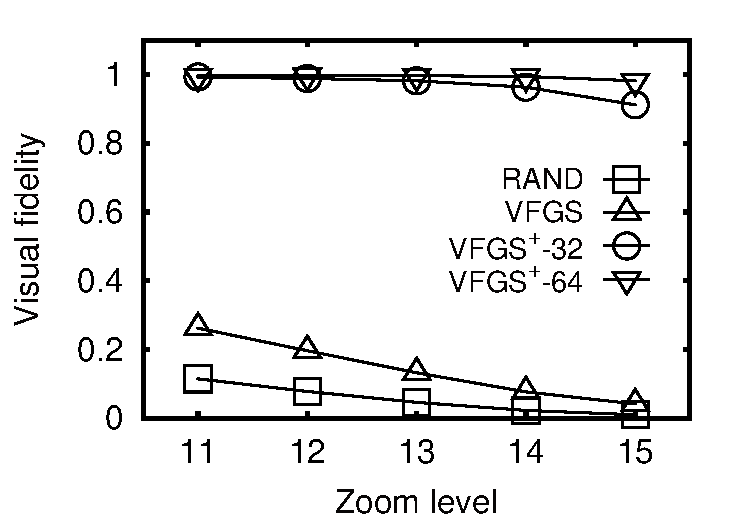
\includegraphics[width=0.44\columnwidth]{pictures/fshenzhen}
   \\
   (A) \pt{}
   &
   (B) \sz{}
 \end{tabular}
 \vspace{-3mm}
 \caption{Visual fidelity of proposed approaches.}
 \label{fig:fidelity}
 \vspace{-4mm}
\end{figure}

\stitle{Visual fidelity evaluation}
We first evaluate the visual fidelity of our proposed methods.
We measure the visual fidelity of different approaches over the $\full$ by using the $loss()$ function we defined in Section~\ref{sec:def}.
Figure~\ref{fig:fidelity}(A) and (B) show the visual fidelity of $\rand$, $\vats$, $\avats$ with $\delta=32$ and $\avats$ with $\delta=64$ from zoom level 11 to 15 (i.e., overview to detail view) in
\pt{} and \sz{}, respectively.
We can conclude that: (i) $\rand$ approach did not guarantee the visual fidelity of the result;
(ii) even $\vats$ offers theoretical visual fidelity guarantee w.r.t. the optimal sampled result set with a given sampling rate, but it still has room for improving over the $\full$;
(iii) $\avats$ with $\delta=32$ and $\delta=64$ has excellent visual fidelity w.r.t. the $\full$ dataset. The minimum visual fidelity value is 0.95 and 0.91 in \pt{} and \sz{}, respectively.
It also confirms the superiority of our proposal;
and (iv) the visual fidelity of $\avats$ falls with the rising of zoom levels, e.g., from zoom level 11 to 15.
The reason is the higher zoom level, the more details are expected.


\begin{figure}
 \centering
 \small
 \begin{tabular}{cc}
   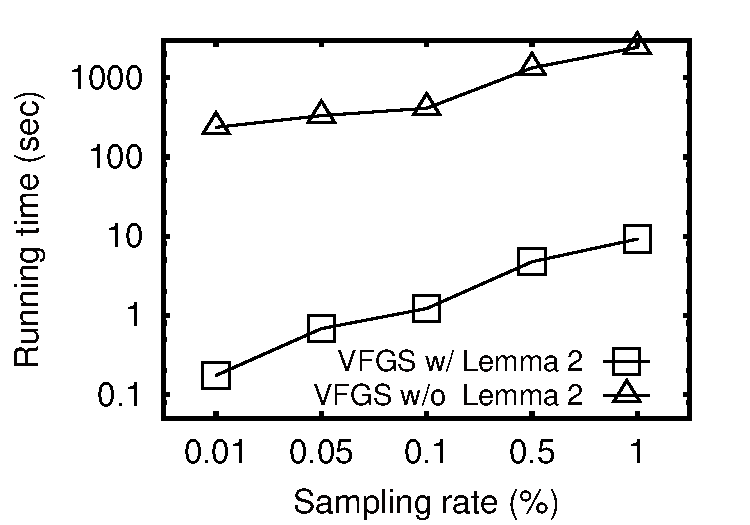
\includegraphics[width=0.44\columnwidth]{pictures/tporto}
   &
   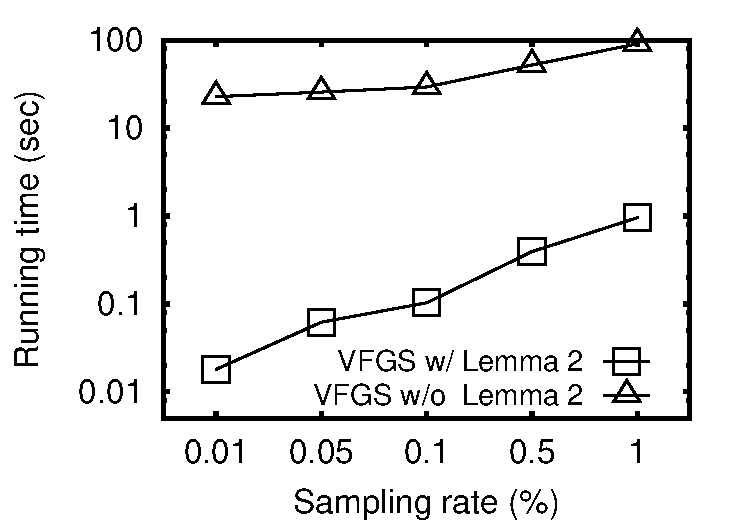
\includegraphics[width=0.44\columnwidth]{pictures/tshenzhen}
   \\
   (A) \pt{}
   &
   (B) \sz{}	
 \end{tabular}
 \vspace{-3mm}
 \caption{The running time of $\vats$ with or without Lemma~\ref{lem:submodular}.}
 \label{fig:cost}
 \vspace{-4mm}
\end{figure}


\stitle{Running time evaluation}
Last, we report the running time of our $\vats$ on two datasets: \pt{} and \sz{} by varying the sampling rate from $0.01\%$ to $1\%$.
It is no doubt $\vats$ is quite slow without the submodularity of contribution value, see Lemma~\ref{lem:submodular} in Section~\ref{sec:opt}.
Our optimized $\vats$ (e.g., $\vats$ with Lemma~\ref{lem:submodular}) outperforms $\vats$ by one to three orders of magnitudes in both \pt{} and \sz{}, as shown in Figure~\ref{fig:cost}(A) and (B).
Finally, with the excellent performance of our $\vats$, we conclude that our proposals support interactive visualization for large trajectory data exploration, i.e., they generate visualization results within seconds.




\section{Conclusion and future work}\label{sec:con}
%Visualizing large trajectory dataset is challenge due to two reasons: visual clutter and long rendering time.
%Data sampling technique, an effective method in reducing the rendering time by shrinking the data size, has been applied in a variety of data.
%However, very few work target at the trajectory sampling especially from the perspective of visualization.
%The most commonly used sampling method, uniform random sampling technique, always generate results with very poor visual quality because very few trajectories located at margin regions can be preserved.
%We fill the gap by proposing a novel sampling techniques $\avats$ which guarantees the visual quality at overview and reduce the visual clutter at the detail view. The technique characteristics and a series of parameters setting are discussed.
%We compare $\avats$ with uniform random sampling in regarding to visual quality preservation and time-usage. We evaluate the effectiveness of proposed method by applying our method to different dataset and conducting users studies on specific interactive trajectory exploration tasks.
%Even though it is recommended to use our method with caching techniques, our experience in the experiment shows that a faster algorithm will be more user friendly for the real world ad-hoc exploration tasks. For future work, we first plan to reduce the time usage by leveraging the advanced database techniques such as the indexing technique or use GPU acceleration.
%In addition, there are several directions can be further explored to enrich the information presented by the visualization.
%First we will develop different color encoding schema to present the spatial distribution of trajectory more precisely.
%In current schema, the color of one trajectory is the same, thus the color of the long trajectories may mislead the users because they pass  through many regions with different level of the traffic crowdedness. One solution is to use gradient color schema to encode the trajectories.
%Another interesting direction is to extend the approach to support the mulit-class characteristics which is a commonly existed in variety of trajectory dataset.
In this paper, we present a novel sampling {technique} $\avats$ which guarantees the visual fidelity at overview and reduce the visual clutter at the detail views.
We evaluate the effectiveness of the proposed method by applying our approaches to different dataset and conducting extensive user studies on three trajectory exploration tasks.
There are several promising future directions, e.g., (i) improving the visual fidelity by considering the trajectory segments sampling instead of the whole trajectories;
and (ii) developing advance color encoding schemas to present the spatial distribution of trajectories more precisely.
%extending our approaches to support the specific trajectory features such as mulit-class characteristics.

%we focus on the sampling approach of trajectory segments other than the whole trajectories to achieve higher visual fidelity.
%We will also develop different color encoding schema to present the spatial distribution of trajectories more precisely. Currently, the color of one trajectory keep the same, thus the color of the long trajectories may mislead the users because they may pass through many regions with different traffic crowdedness.
%We also consider to extend our approach to support the specific trajectory features such as mulit-class characteristics. 



%\begin{acks}
% This work was supported by the [...] Research Fund of [...] (Number [...]). Additional funding was provided by [...] and [...]. We also thank [...] for contributing [...].
%\end{acks}


\bibliographystyle{ACM-Reference-Format}
\bibliography{ref}

\end{document}
\endinput
